\newpage

\section{Post-Inflation}
\label{reheating}


This section refers to physics that originates between the end of inflation and the start of the thermal Hot Big Bang. It begins with the universe still dominated by the vacuum energy of inflation, but now moving away from slow-roll as the inflationary epoch terminates. It ends as the universe settles into the Hot Big Bang: a radiation-dominated epoch with the energy density predominantly in relativistic thermalised Standard Model degrees of freedom. In this section, we focus on what happened between these two eras. This is not a comprehensive review of all aspects of cosmology in this epoch. Instead, we focus on those aspects where stringy physics is especially relevant. Readers interested in a more general treatment of the standard cosmology can consult e.g. \cite{Kolb:1990vq, Baumann:2022mni}, while an earlier discussion of aspects of moduli physics in this epoch is \cite{150207746} and a review of non-standard expansion histories is \cite{Allahverdi:2020bys}.
 
 While it is true that there exists a `standard' cosmological account of reheating, involving a rapid transfer of energy from inflationary degrees of freedom to relativistic Standard Model degrees of freedom, in string theory cosmologies there are no strong reasons to expect this standard account to hold. Although some aspects of the standard cosmology may be preserved in some string theory models, the standard cosmology may be modified in (at least) three ways. First, through the existence of large field displacements between the end of inflation and the final vacuum. Second, in there being no necessary relationship between the inflaton field and the field responsible for reheating. Third, through the expectation of a long moduli-dominated epoch in the universe culminating in moduli-driven reheating. These possibilities are illustrated in Fig. \ref{ReheatingCartoon}. In addition, UV complete string models may connect aspects of early universe and particle physics that otherwise appear uncorrelated.
 
\begin{figure}[ht]
\centering
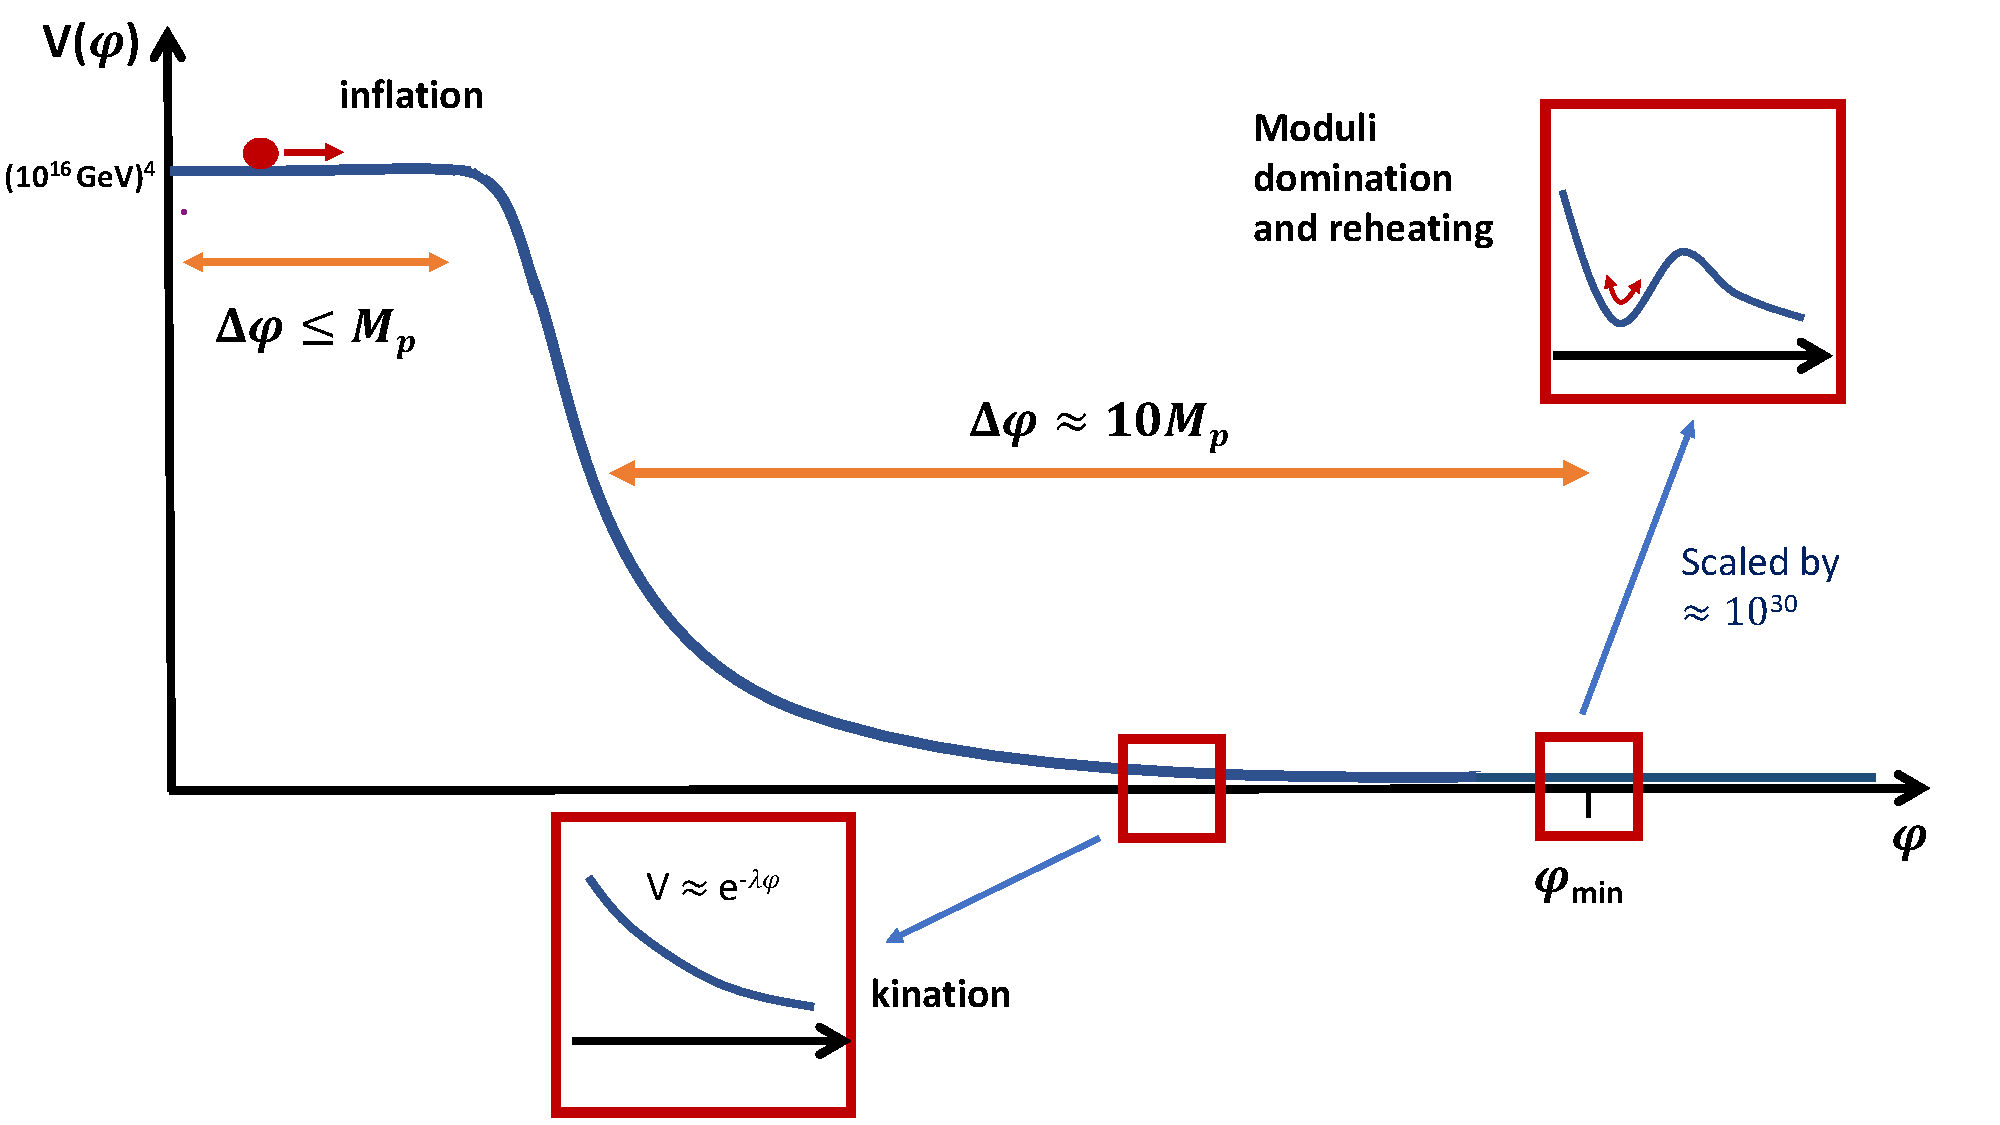
\includegraphics[width = 0.9\textwidth]{Sections/Figures/InflationKinationMD.pdf} 
\caption{A cartoon of one way moduli and stringy physics can substantially modify the post-inflationary history of the universe. Following a period of inflation at relatively high energies, several epochs may occur prior to the start of the Hot Big Bang. We show here the case of a kination epoch followed by moduli domination leading to late reheating. Note the large range of scales that may arise in the scalar potential and the scalar 
field displacement. In particular, the barrier after the minimum may be $20$ (or more) orders of magnitude smaller than the energy scale during inflation ($V_{\rm barrier}\simeq 10^{-20} V_{\rm inf}$).}
\label{ReheatingCartoon}
\end{figure}

\subsection{The Standard Cosmology}

We start with a brief review of the `standard' account of post-inflationary cosmology. During the inflationary epoch, the universe was dominated by the vacuum energy density of a scalar field and the evolution of the universe was well approximated by
\begin{eqnarray}
H(t) & = & H_{\rm inf}\,,  \\
a(t) & = & a(t_{\rm init})\, e^{H_{\rm inf}(t - t_{\rm init})}\,,  \\
\rho(t) &=& V_{\rm inf} = 3 H_{\rm inf}^2 M_{\rm Pl}^2\,.
\end{eqnarray}
During inflation, the inflaton slowly rolls down a flat potential. As inflation ends, the inflaton starts rolling rapidly and oscillates about the minimum of the potential. The amplitude of the inflaton $\phi$ can be modelled by
\begin{equation}
\label{infdecay}
\setlength\fboxsep{0.25cm}
\setlength\fboxrule{0.4pt}
\boxed{
\ddot{\phi} + (3 H + \Gamma) \dot{\phi} = - m^2 \phi\,.
}
\end{equation}
Strictly, Eq. (\ref{infdecay}) is only correct if the inflaton is oscillating rapidly about its minimum.

The coherent oscillations of the inflaton are equivalent to a population of massive inflaton quanta. These quanta behave as massive particles and decay to the Standard Model
with a decay rate $\Gamma$ and with a lifetime $\tau \equiv \Gamma^{-1}$. For times $t \ll \tau$ the universe is matter-dominated and 
filled by $\phi$ particles. It evolves as
\begin{eqnarray}
a(t) & = & a(t_{\rm init}) \left( \frac{t}{t_{\rm init}} \right)^{2/3}\,, \\
\rho(t) & = & \frac{\rho_{\rm init}}{a^3}\,.
\end{eqnarray}
For times $t \gg \tau$, all $\phi$ particles have decayed, and the universe is radiation-dominated, leading to
\begin{eqnarray}
a(t) & = & a(t_{\rm init}) \left( \frac{t}{t_{\rm init}} \right)^{1/2}\,,  \\
\rho(t) & = & \frac{\rho_{\rm init}}{a^4}\,.
\end{eqnarray}
At this point, reheating has fully occurred and there is no energy density left in the inflaton field, with all energy transferred to the Standard Model. While nothing in the above specifies the lifetime $\tau$ which marks the transition into the Hot Big Bang, it is normally expected to be short, lasting for few or no e-folds in the scale factor.

In a full treatment, the process of reheating is time-dependent as decays are stochastic and governed by quantum mechanics.
However, an analytically simple approximation which captures most of the relevant physics is the \emph{instantaneous decay approximation}. In this approximation, all inflaton particles are assumed to decay at the same time $\tau$, at which $H = H_{\rm dec}$. As $H = 1/(2t)$ during radiation domination, $H_{\rm dec} = \Gamma/2$.

As the energy density of thermalised radiation is set as
\begin{eqnarray}
\rho_\gamma & = & \frac{\pi^2}{30} g_* T^4\,, \\
V & = & 3 H^2 M_{\rm Pl}^2\,,
\end{eqnarray}
we can evaluate the reheating temperature as $V_{\rm dec} = 3 H_{\rm dec}^2 M_{\rm Pl}^2$, to obtain
\begin{equation}
\setlength\fboxsep{0.25cm}
\setlength\fboxrule{0.4pt}
\boxed{
T_{\rm rh}^4 = \frac{90}{g_* \pi^2}\,H_{\rm dec}^2 M_{\rm Pl}^2\,.
}
\end{equation}
This formula defines the reheat temperature, corresponding to the last stage of significant entropy injection. The subsequent evolution of the universe is a radiation-dominated Hot Big Bang. 

The reheating temperature specifies the maximum temperature at which the formalism of a thermalised Hot Big Bang can be applied. The actual value of the reheating temperature is crucial for many questions in particle cosmology and astroparticle physics. For example, scenarios of thermal leptogenesis rely on reheating temperatures $T_{\rm rh} \gtrsim 10^{11}\,\rm{GeV}$, whereas many scenarios of dark matter production, such as thermal freeze-out, involve $T_{\rm rh} \gtrsim 1\,\rm{GeV}$. Nonetheless, the only \emph{strong} constraint is that reheating must occur prior to the time when nucleosynthesis commences ($t \sim 0.01\,\hbox{s}$, $T_{\rm BBN} \sim 1 \, \rm{MeV}$). Once the Hot Big Bang starts, the subsequent evolution of the universe is well approximated by
\begin{eqnarray}
a(t) & = & a(t_{\rm init}) \left( \frac{t}{t_{\rm init}} \right)^{\frac12}\,, \nonumber \\
\rho(t) & = & \frac{\pi^2}{30} g_* T^4\,.
\end{eqnarray}
Here $T$ denotes the thermalised temperature and $g_*$ the effective number of relativistic degrees of freedom
\begin{equation}
g_* = \sum_{\rm bosons} g_{\rm b}  + \frac78 \sum_{\rm fermions} g_{\rm f}\,.
\end{equation}

In the `standard' treatment of reheating, it is normally assumed that the inflaton will decay (and reheat the universe) via tree-level perturbative couplings to the Standard Model, e.g. 
\begin{equation}
y \phi \bar{Q} Q\,,
\label{infperd}
\end{equation}
where $y$ is the Yukawa coupling, analogous to the couplings of the Standard Model Higgs ${\cal H}$. For such perturbative decay channels, the decay rate is
\begin{equation}
\Gamma_\phi \sim \frac{y^2}{16 \pi} m_\phi\,.
\label{renormdecay}
\end{equation}
If the inflaton decays via perturbative and renormalisable channels, as in Eq. (\ref{infperd}) above, then
\begin{equation}
\setlength\fboxsep{0.25cm}
\setlength\fboxrule{0.4pt}
\boxed{
T_{\rm rh} \sim  \left( \frac{y^2}{16 \pi} m_\phi M_{\rm Pl} \right)^{\frac12}\,.
}
\end{equation}
For $m_\phi \gtrsim 1\,\hbox{TeV}$, the resulting reheat temperature is rather large; such large reheat temperatures are necessary for various Beyond-the-Standard-Model scenarios such as thermal leptogenesis.

In string cosmologies, we expect substantial modifications to this picture, both in terms of the physics of reheating and also in terms of the evolution of the fields between the end of inflation and the final minimum. The latter is chronologically earlier and so we consider it first. 
In doing so, we are compelled to consider a problem associated to a tension between inflationary and Standard Model energy scales.

\subsection{The Overshoot Problem}

As described in Sec. \ref{ModuliSection} the field space of string compactifications is described by moduli which can vary across many Planckian distances in their expectation values. There is no reason that the present day vacuum of the theory should occupy a similar location in moduli space now 
as it did during the inflationary epoch; indeed, they may be separated by many Planckian distances in field space. In that case, the theory has to move in moduli space from one location to the other. As with other similar points in this section, this is not a \emph{necessary} feature of models of string inflation; however, our focus here is on the novel behaviours that can occur in string cosmology, rather than the cases where a string cosmology replicates more standard scenarios.

Such a cosmological evolution can give rise to a dynamical problem. As detailed in Sec. \ref{sec:infla}, inflation is the leading candidate theory that can simultaneously explain both the large-scale homogeneity of the universe and the presence of small-scale inhomogeneities which have subsequently grown into galaxies and the other cosmic structures we see today. Inflation is characterised by an exponential growth in the scale factor of the universe driven by the vacuum energy of a scalar field. The rate of this growth arises from the size of the vacuum energy during inflation. While not yet known, it is naturally large. Expressed in terms of the tensor-to-scalar ratio $r$ which stage 4 CMB experiments hope to measure, it is
\begin{equation}
V_{\rm inf}^{1/4} \sim r^{1/4}\, 10^{16}\, \rm{GeV}\,.
\end{equation}
However, the quasi-de Sitter state experienced during inflation is, by definition, not the final vacuum and string theory/supergravity models of inflation typically end with rolling moduli.

During the inflationary epoch, we expect the characteristic scales to be large. In supergravity models, unless special and specific cancellations occur, the scale of the potential is $V \sim m_{3/2}^2 M_{\rm Pl}^2$. This follows from
\begin{equation}
V = e^K \left[ K^{i\bar{\jmath}} D_i W D_{\bar{\jmath}} \overline{W} - 3 \vert W \vert^2 \right]
\end{equation}
and $m_{3/2} = e^{K/2} \vert W \vert$ (in units where $M_{\rm Pl} = 1$). Based on this, for $r \gtrsim 10^{-12}$ (as holds in essentially all models of inflation) we expect the gravitino mass during inflation to satisfy $m_{3/2} \gtrsim 10^9 \, \rm{GeV}$.

The key point is that when inflation ends, the state of the universe is \emph{likely to involve rolling moduli fields, with potential energies far greater than any of those currently applicable in particle physics}. The cosmological evolution must take us from this state to the current vacuum, in the process dissipating all this early potential energy. 

The overshoot problem is the question of why, and how, this evolution ends up in the current vacuum, as opposed to simply running off to the 10-dimensional decompactification limit. In terms of the 4-dimensional effective potential, it is always the case that $V \to 0$ 
in the asymptotic limits where $g_s \to 0$ or $\mathcal{V}_s \to \infty$ at the boundary of moduli space. This can be seen in several ways, but the most intuitive is to note that since the string scale relates to the 4-dimensional Planck scale as (where $\mathcal{V}_s$ is the volume of the Calabi-Yau measured in units of $l_s^6$ in terms of the 10-dimensional string frame metric in the convention where string and Einstein frame metrics coincide in the vacuum\footnote{The relation between the metrics in string and Einstein frames in 10 dimensions is convention dependent and in general is given by  $G_{MN}^S = e^{\frac{\phi-\phi_0}{2}}G_{MN}^E$, the above choice of conventions corresponds to 
$\phi_0= \langle \phi \rangle$. Note that this differs from the convention used in the moduli stabilisation section.})
%
\begin{equation}
\label{convvvv}
\setlength\fboxsep{0.25cm}
\setlength\fboxrule{0.4pt}
\boxed{
M_s = \frac{g_s}{\sqrt{4\pi}}\frac{M_{\rm Pl}}{\sqrt{\mathcal{V}_s}}\,,
}
\end{equation}
then in 4-dimensional Einstein frame these asymptotic limits correspond to $M_s \to 0$. As all physical scales in string theory (including the scalar potential) depend on $M_s$, as $M_s \to 0$ it will always be the case that $V \to 0$.

If post-inflationary evolution starts with the universe having large positive vacuum energy in the deep interior of moduli space, why does it not just evolve so that it runs away all the way to the zero-potential decompactification limit? (see Figure \ref{Fig:Kination}).

As the current vacuum is a local minimum of the potential, it is surrounded by a barrier to decompactification. However, the height of this barrier is typically  $\sim m_{3/2}^2 M_{\rm Pl}^2$ (following from the general structure of the supergravity scalar potential), and many scenarios assume $m_{3/2}^{\rm now} \ll m_{3/2}^{\rm inf}$. A primary example where $m_{3/2}^{\rm now} \ll m_{3/2}^{\rm inf}$ is explicitly realised is when inflation is driven by the volume modulus close to an inflection point at small field values \cite{Conlon:2008cj, Cicoli:2015wja}. The height of the barrier is minuscule compared to the height of the original potential -- so how can the barrier trap the fields? To visualise this problem, one can imagine a rollercoaster released under gravity from a height of a hundred metres and which must stop at an endpoint where the track rises by one millimetre -- except the inflationary case involves a far greater disproportion in the relative potential heights.

The overshoot problem was first formulated by Brustein and Steinhardt \cite{Brustein:1992nk}. A key point of their analysis, which remains true today, is that stringy potentials are naturally extremely steep. To appreciate this, note that the two most important moduli are the dilaton ($S$) and volume modulus ($T$), as these incorporate $g_s$ and $\mathcal{V}$ and so control the asymptotic runaway limit to large volume and weak coupling. The K\"ahler potential is logarithmic in these moduli, typically
\begin{equation}
\setlength\fboxsep{0.25cm}
\setlength\fboxrule{0.4pt}
\boxed{
K = - \ln \left(S + \bar{S} \right) - 3 \ln \left( T + \overline{T} \right).
}
\end{equation}
Examining the metric $K_{S\bar{S}}$ or $K_{T\overline{T}}$, this implies that the \emph{canonically normalised} field is logarithmic in either the string coupling $g_s$ or the volume $\mathcal{V}$.

Any string-derived potential that is a simple power-law in the dilaton or volume -- as would arise from any perturbative weak coupling expansion in either $g_s$ or $\alpha'$, or also any potential whose natural scaling is $M_s^4$ -- will then correspond to a potential that is a runaway exponential in the canonically normalised field $\phi$, $V(\phi) \propto e^{-\lambda \phi}$. Note that while such a runaway exponential cannot itself have a minimum, it may nonetheless be a good approximation to the moduli potential over a large region of its field range, and so be a good approximation to the full potential.

Such an exponential potential
\begin{equation}
V(\phi) \propto e^{-\lambda \phi}
\end{equation}
is already rather steep. We note that in string theory `flat' exponentials do not occur; current evidence 
suggests that $\lambda > \sqrt{2}$ and accelerated expansion cannot occur (e.g. see \cite{Garg:2018zdg, Olguin-Trejo:2018zun, ValeixoBento:2020ujr, Cicoli:2021fsd, Rudelius:2022gbz, Calderon-Infante:2022nxb, Shiu:2023nph} for recent discussions).

Moreover, in many cases stringy potentials actually arise from non-perturbative terms in the superpotential: examples are gaugino condensation in racetrack models, or the non-perturbative effects in KKLT. For such models the potential in terms of the canonical field is instead a double exponential:
\begin{equation}
V(\phi) \propto e^{-\alpha e^{\beta \phi}}\,.
\end{equation}
Like a second slice of chocolate cake, this is perhaps too much of a good thing; manifestly, such double exponentials are exceptionally steep
and, plotted on a linear axis, resemble a vertical cliff -- which simply serves to re-emphasise the overshoot problem.

\subsection{The Road to a Solution: Rolling and Tracker Solutions}

The overshoot problem is a well-posed question about the immediate dynamics of post-inflationary string cosmology. It looks like a sharp and severe problem. However, it turns out there is a clear roadmap to a solution which also offers the attractive possibility of quasi-universal behaviour in the early universe (within the context of string compactifications). First, however, we describe the simplest solutions to the overshoot problem (but also ones which remove most of the interesting physics from it).

The overshoot problem exists when the scales present in inflation are substantially larger than the scales of the barrier preventing decompactification. If this is not the case, then there is clearly no overshoot problem. There are two easy ways to achieve this but both are somewhat artificial. The first is through models of extremely low scale inflation. If $V_{\rm inf} \sim \left( 1\, {\rm TeV} \right)^4$, then the inflationary potential is comparable to the weak scale and there is no overshooting problem to explain (for example, see \cite{hepph0103243, 09122324}).
However, it is difficult to embed such models into string theory as viable UV-complete examples of inflation.

The second `trivial' solution to the overshoot problem is to require that the scales of the post-inflationary vacuum are the same as that of the inflationary potential. The barrier height is then, automatically, comparable to the scale of the potential during inflation. In this case, there would be manifestly no overshoot problem. Examples of models utilising this approach are \cite{0411011, 0611183, 11124488}. The problem with this solution (and why we use the word `trivial' to refer to it) is that it ducks the question of where the weak scale (or indeed, any of the other particle physics hierarchies) actually comes from. While it is intellectually consistent to regard the weak scale as a pure accident of nature, arising from either a highly fine-tuned Standard Model or a similarly fortuitous cancellation resulting in a light gravitino mass (i.e. $m_{3/2}^2 \ll m_\phi^2$ from fine-tuning), this avoids all the deep `why' questions about the Standard Model and its energy scales. One can then reasonably  ask: why care about using string theory in the first place to understand the hierarchy problems of the Standard Model?

Another approach to mitigate the overshoot problem comes from cases where the Standard Model is 
sequestered from the sources of supersymmetry breaking, since in this case low-energy supersymmetry could be compatible 
with a large gravitino mass. However, such sequestering requires a particular realisation of the Standard Model with D3-branes at singularities and several sources of desequestering can ruin this picture e.g.~\cite{Conlon:2010ji, Berg:2012aq}. Moreover, even in the presence of sequestering, TeV-scale supersymmetry can be compatible with at most $m_{3/2}\sim 10^{11}$ GeV, which would still be 3 orders of magnitude smaller than a Hubble scale during inflation of order $H_{\rm inf}\sim 10^{14}$ GeV. Such scenarios would, therefore, likely still have some remnant overshoot problem to be solved.



A more attractive and more ambitious solution to the overshoot problem (compared to the above) comes from the ideas of kination epochs and tracker solutions. To see how these arise, we start with the equations of motion for an evolving scalar:
\begin{subequations}
\label{fgha1}
\begin{empheq}[box=\widefbox]{align}
\ddot{\phi} + 3H\dot{\phi} & =  - \frac{\partial V}{\partial \phi}\,, \\
H^2 & = \frac{1}{3 M_{\rm Pl}^2} \left( V(\phi) + \frac{\dot{\phi}^2}{2} \right).
\label{fgha2}
\end{empheq}
\end{subequations}
The Hubble friction term (proportional to $H$) implies that all sources of energy act as friction on a scalar rolling down a potential. If large enough, this braking friction will avoid the overshoot, by slowing down the scalar sufficiently so that it fails to climb over the barrier to decompactification. While there are contributions to Hubble friction from both the potential itself and any kinetic energy of the scalar field, the self-braking is not by itself enough to avoid overshoot.
\begin{center}
\begin{figure}
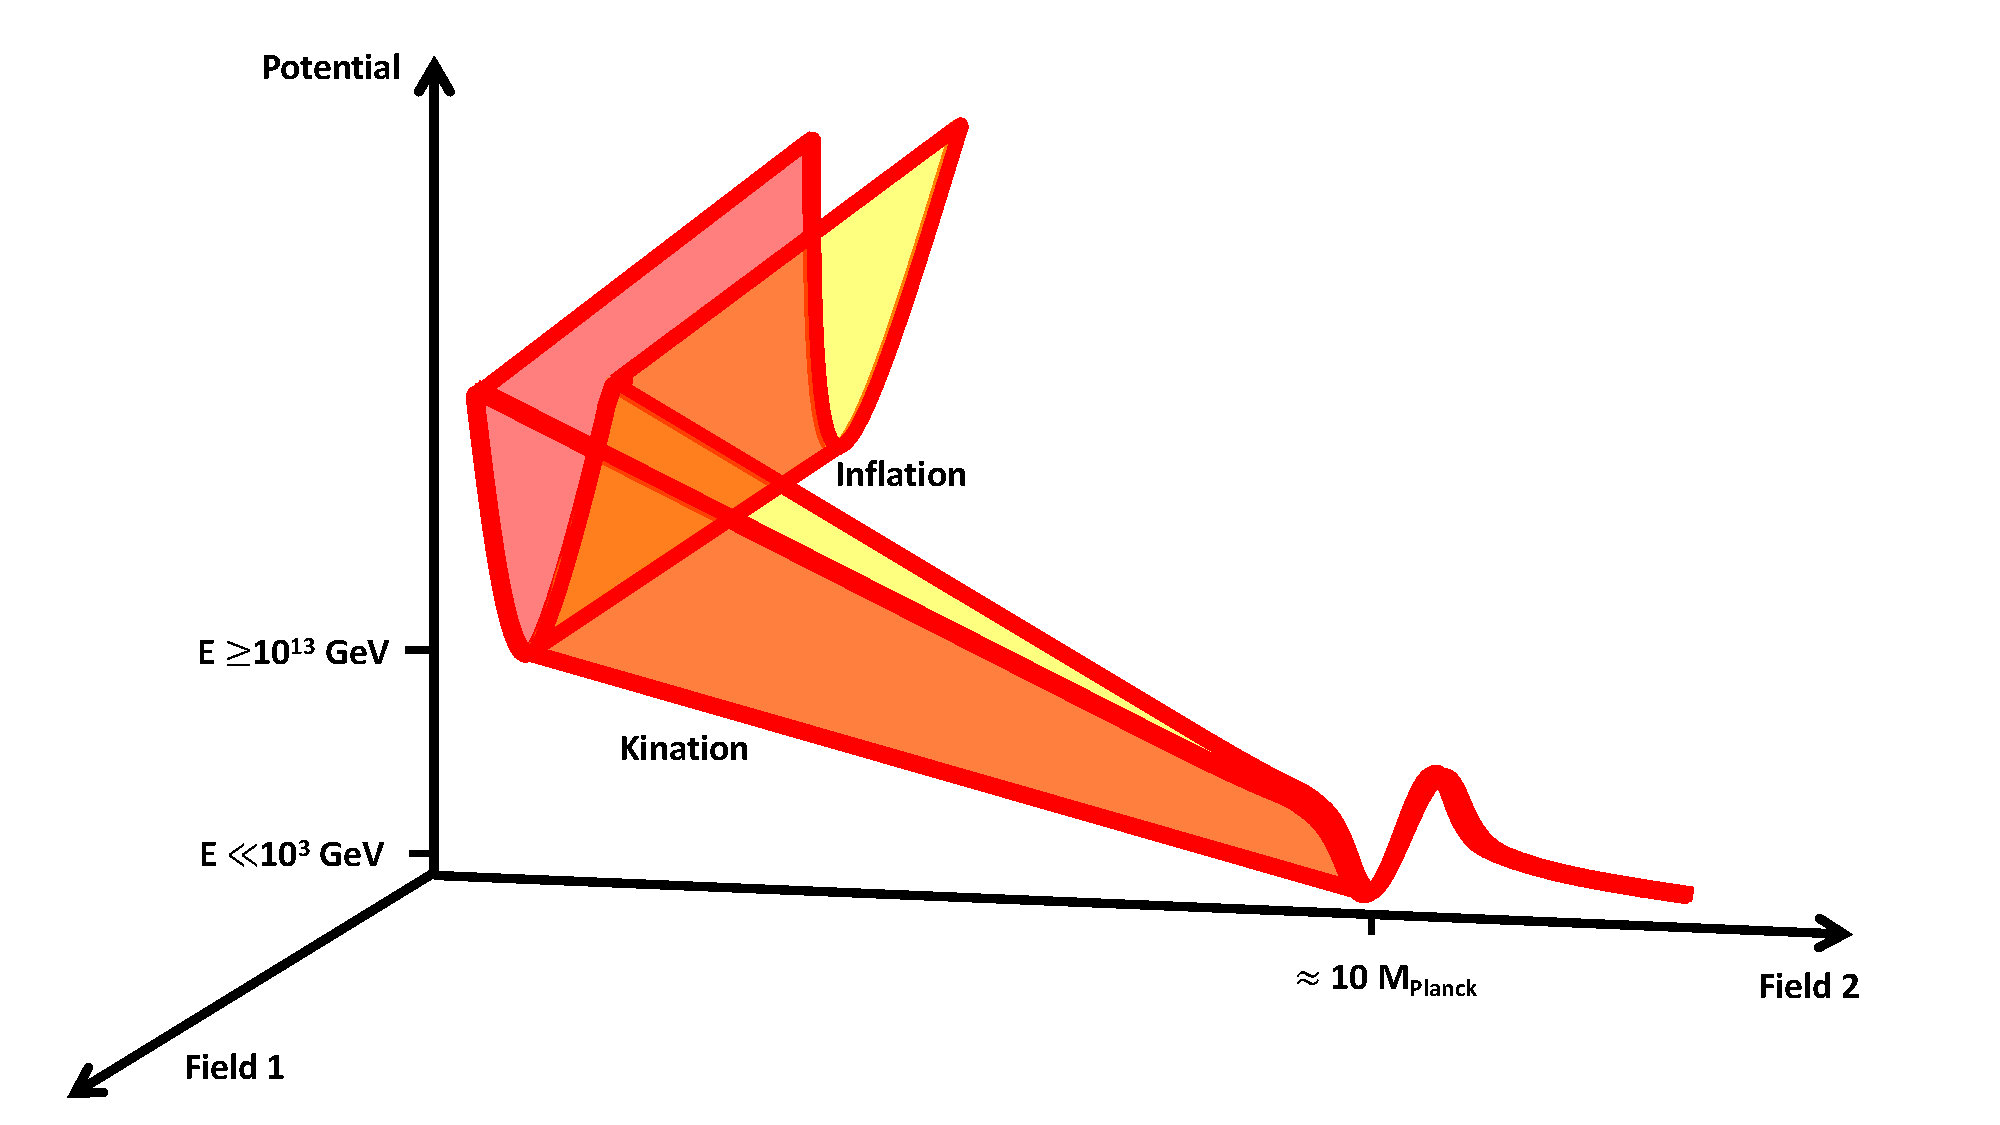
\includegraphics[width=14cm]{Sections/Figures/Kination3.pdf}
\caption{A typical potential featuring high scale inflation and a low barrier toward decompactification which can potentially suffer from the overshoot problem. Figure by Elisa Quevedo.}
\end{figure}
\label{Fig:Kination}
\end{center}
In slow-roll inflation, the largest contribution to $H$ is the energy density in the potential. However, once a field starts rolling down an exponential (or even double-exponential) slope, the steepness of the potential implies that the kinetic energy of the inflaton rapidly becomes large. In particular, 
it dominates over the contributions of the potential density. The universe then enters a phase where its energy density is dominated by the kinetic energy of the scalar field -- a \emph{kination} phase (first named in \cite{hepph9606223}). For a recent review of kination, see \cite{211101150}.

In such a kination epoch, the scalar field equations of motion Eq.~(\ref{fgha1}) and (\ref{fgha2})
reduce to 
\begin{eqnarray}
\ddot{\phi} + 3H\dot{\phi} & =  & 0\,, \\
H^2 & = &  \frac{\dot{\phi}^2}{6 M_{\rm Pl}^2}\,.
\label{HEq}
\end{eqnarray}
This results in an equation for $\phi$:
\begin{equation}
M_{\rm Pl} \, \ddot{\phi} + \sqrt{\frac32}  \dot{\phi}^2 = 0\,,
\end{equation}
which is solved by 
\begin{equation}
\label{fieldkination}
\setlength\fboxsep{0.25cm}
\setlength\fboxrule{0.4pt}
\boxed{
\phi = \phi_{\rm init} + \sqrt{\frac23} M_{\rm Pl} \ln \left( \frac{t}{t_{\rm init}} \right).
}
\end{equation}
Here the initial condition has been set as $\phi(t_{\rm init}) = \phi_{\rm init}$. The residual integration constant has been fixed by requiring that a time coordinate of $t=0$ represents (at least formally) an initial singularity where the energy densities diverge. It is worth noting that during kination, the field moves through approximately one Planckian distance in field space each Hubble time. 
This is an interesting feature from the perspective of \emph{string} cosmology; such trans-Planckian field excursions are home territory for string theory and require a theory of quantum gravity to ensure adequate control of the effective field theory expansion over such large displacements. Any extended kination epoch, lasting for many Hubble times, will result in a field traversing a markedly trans-Planckian distance (such a kination epoch can also have an interpretation as a 10-dimensional Kasner solution \cite{Apers:2022cyl}).

The scale factor behaves as
\begin{equation}
a(t) \propto t^{1/3}\,,
\end{equation}
which follows immediately from $H^2 \equiv \left(\frac{\dot{a}(t)}{a(t)}\right)^2 = \frac{\dot{\phi}^2}{6 M_{\rm Pl}^2}$. During a kination epoch, the energy density  therefore drops off as
\begin{equation}
\setlength\fboxsep{0.25cm}
\setlength\fboxrule{0.4pt}
\boxed{
\rho_{\rm kin}(t) \propto a(t)^{-6}\,.
}
\end{equation}
By comparing with $\rho \propto a^{-3}$ or $\rho \propto a^{-4}$ (behaviours of matter and radiation domination), we see that kinetic energy dilutes much faster. This implies that during a fast-rolling kination phase, any initial sources of matter or radiation will -- over time -- catch up with the kination energy. At this point, their additional Hubble friction can effectively stop the evolution of the field (it becomes overdamped) until the energy densities of the universe have fallen sufficiently for the slope of the potential to become important again.

At this point, the evolution enters an attractor tracker solution. The `attractor' nature refers to the fact that many initial conditions converge onto the same solution. The `tracker' property refers to the fact that
fixed proportions of the energy density lie in each of potential energy, kinetic energy and radiation (or matter) \cite{Wetterich:1987fm, Ferreira:1997hj, Copeland:1997et}. The use of tracker solutions, and additional Hubble friction to avoid overshoot, goes back a long way (for example, see  \cite{hepth9805005, hepth0001112, hepph0010102, Barreiro:2005ua, hepth0408160, hepth0505098}).

We now describe the properties of the tracker solution (mostly following the analysis of \cite{Copeland:1997et}).
The existence of the tracker solution relies on the presence additional contributions to energy density that redshift slower than kinetic energy.
For a generic cosmic fluid with equation of state 
\begin{equation}
P= (\gamma - 1) \rho\,, \qquad \qquad \rho \sim a^{-3 \gamma}\,,
\end{equation}
and so a slower redshift than kinetic energy requires $\gamma < 2$. Both matter and radiation satisfy this condition. Given the high inflationary scales, there does not appear to be an obvious candidate for stable matter at the end of inflation (although, as possibilities, one could consider either primordial black holes or relatively heavy axions with $m_a < H$, which become non-relativistic shortly after the end of inflation).

Instead,  we focus on the relatively universal case of initial radiation, where $\rho_{\rm extra} = \rho_\gamma$ (note we use $\rho_\gamma$ to denote any form of radiation, not just photons). There are many good candidates for such radiation (for example, gravitons, axion-like particles or extra $U(1)$ gauge bosons).

The Friedmann equations are
\begin{eqnarray}
\dot{H} & = & - \frac{1}{2 M_{\rm Pl}^2}\Big(\rho_{\gamma}+P_{\gamma} + \dot{\phi}^2\Big) = - \frac{1}{2 M_{\rm Pl}^2} \Big( \gamma \rho_{\gamma}+ \dot{\phi}^2\Big)\,, \\
H^2 & = & \frac{1}{3 M_{\rm Pl}^2}\Big(\rho_{\gamma}+ \frac12\dot{\phi}^2+ V(\phi) \Big)\,,
\end{eqnarray}
with energy conservation set by
\begin{equation}
\dot{\rho}_{\gamma}= -3 H \big( \rho_{\gamma}+P_{\gamma} \big) = -3 H \gamma \rho_\gamma\,.
\end{equation}
The attractor nature is made manifest by transforming to the variables
\begin{equation}
x = \frac{\dot{\phi}}{M_{\rm Pl}} \frac{1}{\sqrt{6} H}\,, \quad \quad y = \sqrt{\frac{V(\phi)}{3}} \frac{1}{M_{\rm Pl} H}\,.
\end{equation}
These variables are equivalent to the fractional energy densities in kinetic and potential energy, $\Omega_k = x^2$ and $\Omega_p = y^2$, while the energy density in radiation is set by $\Omega_{\gamma}= 1- x^2 - y^2$.
The dynamical evolution then becomes
\begin{eqnarray}
  x'(N) &=& -3x - \frac{V'(\phi)}{V(\phi)}\sqrt{\frac32} y^2 + \frac32 x \big[ 2x^2 + \gamma(1-x^2-y^2) \big], \nonumber \\
  y'(N) &=& \frac{V'(\phi)}{V(\phi)}\sqrt{\frac32} xy + \frac32 y \big[ 2x^2 + \gamma(1-x^2-y^2) \big], \label{eq:xy2} \\
H'(N) &=& -\frac32 H (2x^2 + \gamma(1-x^2-y^2)), \nonumber \\
\phi'(N) &=& \sqrt{6} x, \nonumber 
\end{eqnarray}
where the time variable is $N = \ln a$.

One of the simplest possible potentials (which happily also holds for LVS and other models where the potential is power-law in either the dilaton or volume moduli) is where the potential can be approximated by a single (steep) exponential,\footnote{In the context of LVS, the single exponential is a good approximation while the field rolls down the slope. Near the minimum, other terms become important. The full potential takes the form
\begin{equation}
V(\phi)= V_0 \big( (1-\varepsilon \phi ^{3/2}) e^{- \lambda \phi} + \delta e^{- \sqrt{6} \phi }\big)\,. \nonumber
\end{equation}
Here the uplift parameter $\delta$ needs to be fine-tuned to achieve a dS vacuum at $\phi \sim \varepsilon^{-2/3}$. 
}
\begin{equation}
\setlength\fboxsep{0.25cm}
\setlength\fboxrule{0.4pt}
\boxed{
V = V_0\,\exp \left( - \lambda \frac{\phi}{M_{\rm Pl}} \right),
}
\end{equation}
so that $V'(\phi)/ V(\phi) = - \lambda/M_{\rm Pl}$. While in an LVS context, $\lambda = \sqrt{27/2}$, the precise value of $\lambda$ is not essential for the existence of the tracker solution. We regard $\phi = 0$ as corresponding to the central region of moduli space (with either $g_s \sim 1$ or $\mathcal{V} \sim 1$). The precise value of $V_0$ will depend on the details of the compactification, but for reasonable values of $W_0$ we expect it to be of order $M_{\rm Pl}^4$.
In this regime, the system \eqref{eq:xy2} is known to have a stable attractor solution where the scalar field and radiation have a fixed ratio of energy densities. The fixed point is characterised by
\begin{equation}
\setlength\fboxsep{0.25cm}
\setlength\fboxrule{0.4pt}
\boxed{
\Omega_k = x^2 = \frac{3}{2} \frac{\gamma^{2}}{\lambda^{2}}\quad \quad  \Omega_p = y^2 = \frac{3(2-\gamma) \gamma}{2 \lambda^{2}} \quad \quad  \Omega_{\gamma}= 1-x^2-y^2 = 1-\frac{3 \gamma}{\lambda^{2}}\,.
}
\end{equation}
If the attractor solution is obtained before the rolling field reaches the barrier, it will not overshoot.
%

The presence of such attractor solutions has several appealing features. First, it provides a natural \emph{mechanism} for solving the overshoot problem \cite{hepth9805005, hepth0001112, hepph0010102, Barreiro:2005ua, hepth0408160, hepth0505098, 07092810, Conlon:2008cj, 220700567, Alam:2022rtt} (for some alternative approaches, for which we do not have space for a full discussion, see \cite{08073216, 08104251, 10122187, 11124488}). The additional energy content provides a Hubble friction that slows down the rolling runaway field sufficiently to ensure that it does not overshoot the barrier to infinity, but ends in the desired low-energy vacuum. The extra friction provides a natural solution to the overshoot problem, and allows the true vacuum to be located with relative ease.

Second, the required \emph{ingredients} for this mechanism to work -- additional matter or radiation -- are not exotic and are generally present within string compactifications. To be more specific, some extra radiation will always be present at the end of inflation. Associated to the quasi-de-Sitter phase of inflation is a temperature,
\begin{equation}
T_{\rm dS} = \frac{H}{2 \pi}\,.
\end{equation}
The thermal bath associated to this temperature will lead to an energy density in radiation at the end of inflation given by
\begin{equation}
\label{dsenergy}
\rho_{\gamma, {\rm init}} = \frac{\pi^2}{30} g_* \left( \frac{H_{\rm inf}}{2 \pi} \right)^4\,.
\end{equation}
This is a `minimal' level of radiation, as its origin is effectively universal -- whatever the inflationary model, we expect it to be accompanied by thermal background radiation of this magnitude. Other, more model-dependent, sources of inflation include the perturbative conversion of the inflaton degrees of freedom into radiation (i.e.~the analogue of decays in a time-dependent background) or radiation from any cosmic strings that may be formed at the end of inflation, such as in models of brane inflation.

Finally, this mechanism also suggests that an extended period of kination may be a generic, or universal, feature of string cosmology in the early universe: it appears to be a common, if not universal, expectation of string cosmology that the evolution of the universe passes through a kination epoch and then a scaling solution. This would be appealing as it would simplify the search for any distinctive observational footprints from string cosmology: generic behaviour provides a clearer and cleaner target than scenarios where `anything goes'.

All that said, it is also worth enumerating the potential challenges and disadvantages associated to this solution to the overshoot problem. The first such challenge is associated to the large field displacements required. From Eq. (\ref{fieldkination}) we see that during a kination epoch, in every Hubble time the field passes through a Planckian distance in field space. A kination epoch that lasts for a significant number of Hubble times will involve a notably trans-Planckian field excursion. Furthermore, to reach the tracker solution it is likely that such an excursion is necessary; the tracker solution requires radiation to `catch up' with the kinetic energy. However, the nature of inflation is that the initial level of radiation will be highly sub-dominant. For example,  Eq. (\ref{dsenergy}) would give rise to
\begin{equation}
\Omega_{\gamma, {\rm init}} \sim \frac{H_{\rm inf}^2}{M_{\rm Pl}^2}\, .
\end{equation}
The lower the inflationary scale is, the smaller $\Omega_{\gamma, {\rm init}}$ is, and the longer the kination epoch needs to last in order for the radiation to catch up and lock onto the tracker solution.

However, such large field excursions are not without their problems. As reviewed in Sec. \ref{Sec:Swamp}, according to the Swampland Distance Conjecture, towers of states come down in mass whenever a field traverses a trans-Planckian distance $\Delta \phi > M_{\rm Pl}$ \cite{Ooguri:2018wrx},
\begin{equation}
\setlength\fboxsep{0.25cm}
\setlength\fboxrule{0.4pt}
\boxed{
M_i \propto e^{-\alpha \Delta \phi / M_{\rm Pl}}\,,
}
\end{equation}
%
where $\alpha$ is an $\mathcal{O}(1)$ number. Such towers of states may modify the low-energy effective field theory and lead to additional corrections to the Lagrangian, although note that the presence of a descending tower of states is not necessarily a problem: some examples, such as Kaluza-Klein states in the asymptotic large volume regime, are relatively well understood and do not necessarily lead to control issues.

The second, related, challenge is that most possible origins of initial seed radiation generate rather small amounts of radiation, at a level proportional to $\left(H_{\rm inf}/M_{\rm Pl}\right)^2$. For models with low inflationary scales, it would not be possible for fields to reach the tracker solution before they overshoot the barrier and are on their way towards decompactification. In practice, the tracker solution may be hard to locate and in this case, another mechanism to avoid overshoot would have to be found. When the mechanism works, it works well -- but the tracker requires rather specific conditions on the available field displacement in order for it to work.

\subsection{Moduli Domination}

However it happens, overshoot must be avoided in any cosmology that can describe our universe. Sooner or later, the theory must approach our own vacuum and gradually settle into it. It is here that another characteristic aspect of string cosmologies come into play: the expectation of a period of moduli domination. Why?

In expanding universes, matter and radiation redshift as
\begin{subequations}
 \begin{align}\label{matterrad}
    \rho_{\rm mat} & \propto  a(t)^{-3}\,, \\
     \rho_{\rm rad} & \propto  a(t)^{-4}\,,
 \end{align}
\end{subequations}
%
and so matter wins out over radiation.
Although both familiar and basic, Eq.~(\ref{matterrad}) implicitly contains one of the most important elements of \emph{string} cosmology. As discussed in Section \ref{ModuliSection}, moduli originate from higher-dimensional modes of the graviton and interact through gravitationally suppressed couplings. On dimensional grounds, the decay rates of such moduli are set as
\begin{equation}
\setlength\fboxsep{0.25cm}
\setlength\fboxrule{0.4pt}
\boxed{
\Gamma_\phi = \frac{\lambda}{16 \pi} \frac{m_\phi^3}{M_{\rm Pl}^2}\,,
}
\end{equation}
where $\lambda$ is a dimensionless $\mathcal{O}(1)$ constant, whereas particles with renormalisable perturbative decays have decay rates given by Eq. (\ref{renormdecay}). Compared to these, the lifetimes of the scalar moduli are enhanced by a factor of $\left(M_{\rm Pl}/m_\phi\right)^2$. Indeed, as the Planck scale is the silverback mountain gorilla of energy scales in physics, moduli also outlive other particles with non-renormalisable interactions suppressed by (merely) the GUT scale.

When heavy particles decay, their decay products are normally relativistic. With radiation redshifting as $\rho_{\rm rad} \sim a^{-4}$ and matter
redshifting as $\rho_{\rm mat} \sim a^{-3}$, the relativistic products from any `early' decays rapidly grow sub-dominant to any surviving 
matter present.
With the evolution of cosmic time, a universe crowded with particles inevitably becomes dominated by the longest-living, latest-decaying matter. As gravity is, both empirically and theoretically, the weakest force, this implies that it is a generic expectation of string compactifications that the universe will go through a stage where its energy density is dominated by the mass-energy of moduli particles, for which all interactions are non-renormalisable and suppressed by the Planck scale. 

This era of \emph{moduli domination} is one of the most generic and distinctive expectations of string cosmology, and it is one of the most notable ways in which string cosmology differs quite substantially from many field theory approaches to inflation where reheating is assumed to be driven by fields with couplings that are either renormalisable or, at least, suppressed by scales far lower than the Planck scale (see Fig.~\ref{fig:AlternativeHistory}). 

\begin{figure}[ht]
    \centering
    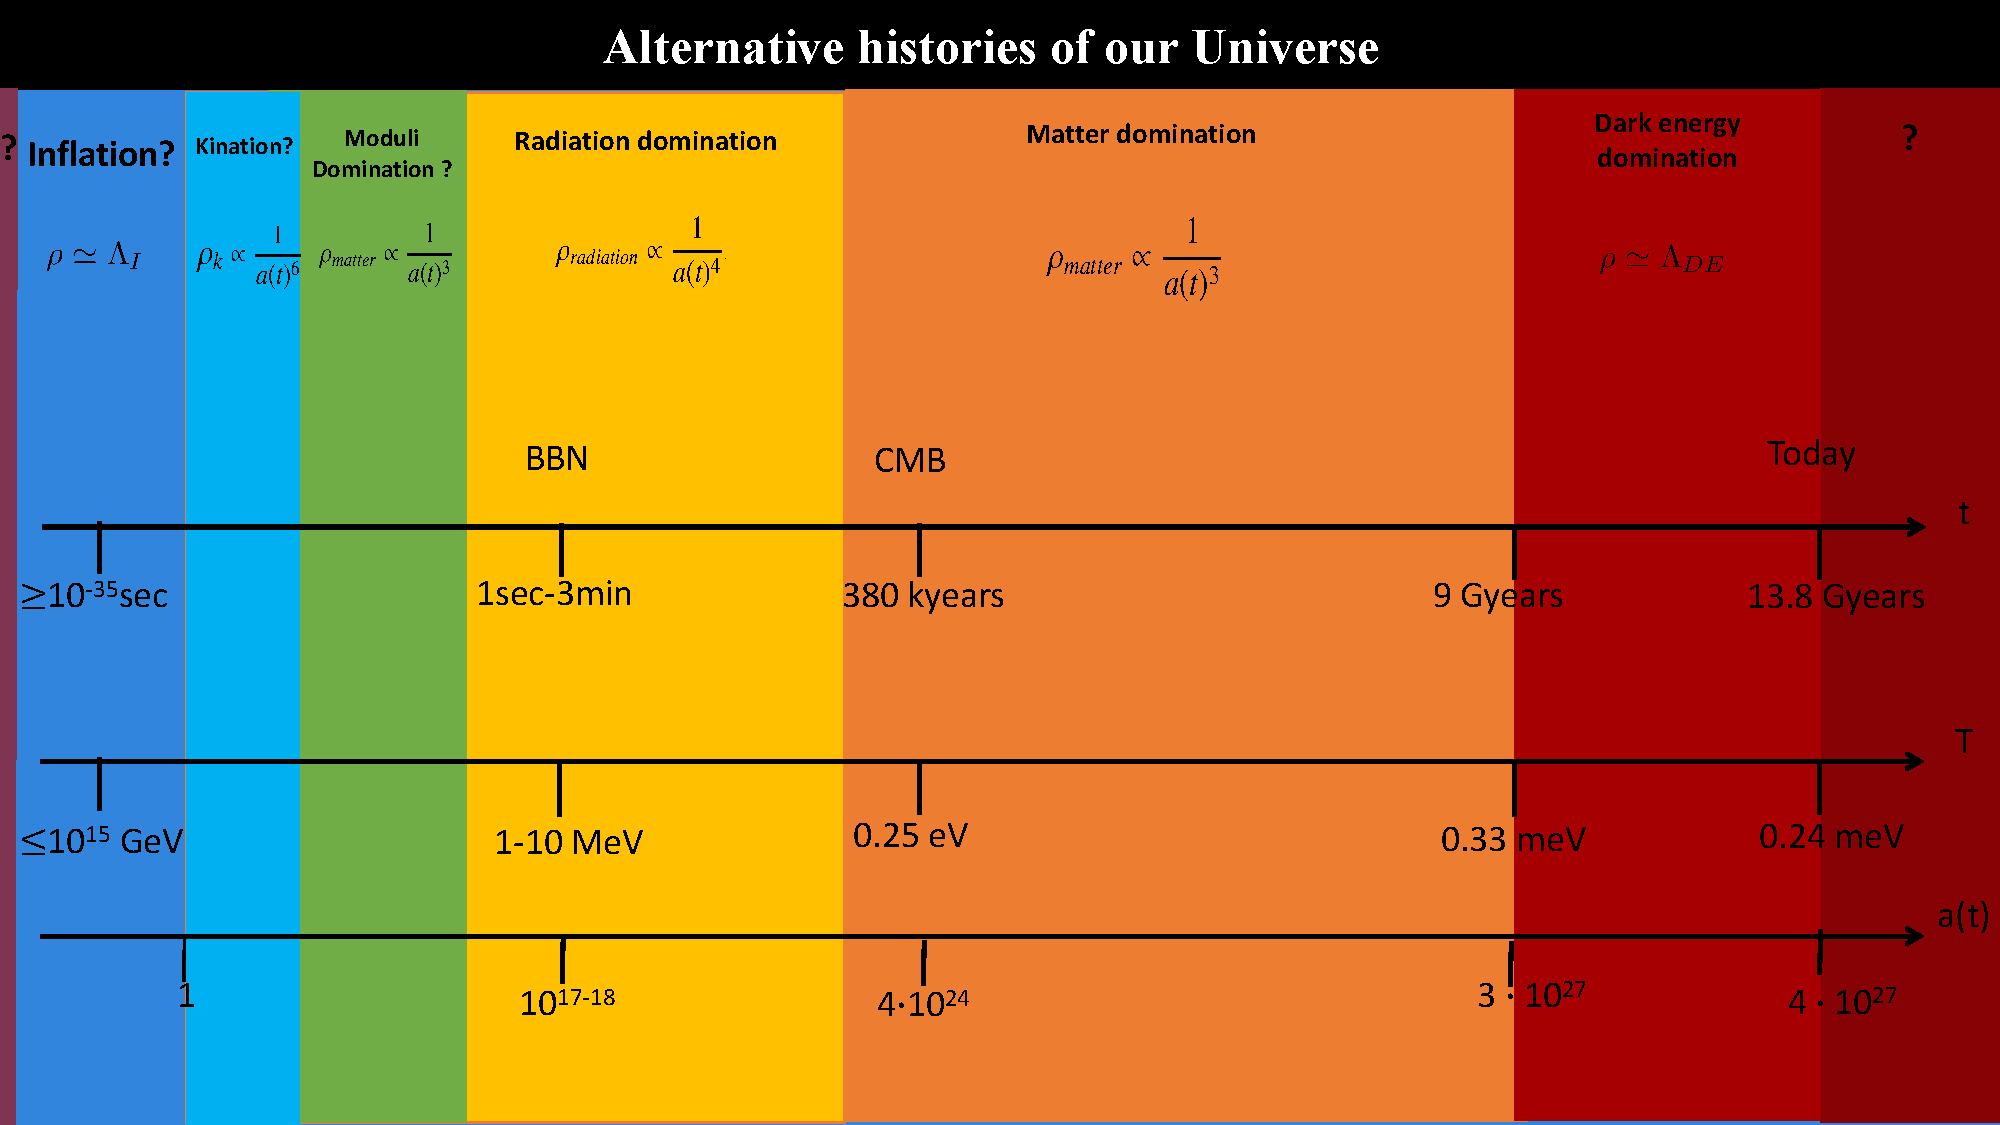
\includegraphics[width = 0.9\textwidth]{Sections/Figures/FigureAlternativeHistory.pdf} 
    \caption{Alternative histories of the universe including potential periods of kination and moduli domination.}
    \label{fig:AlternativeHistory}
\end{figure}

While not strictly unique to string theory (the key feature is the presence of massive scalars with gravitational-strength interactions), it represents a very different cosmological history to many Beyond-the-Standard-Model post-inflationary scenarios, which involve a rapid transfer of energy from the inflationary degrees of freedom into Standard Model particles.

Sometimes string theory is seen as an esoteric UV issue of little interest to hard-working practical cosmologists studying the universe one trillionth of a second after the Big Bang. It is, therefore, important to note that the cosmology of such standard field theory scenarios is unstable to the inclusion of a sector with only gravitationally coupled particles (i.e. moduli). As described above, as long as there is \emph{some} initial amplitude in the moduli fields, we expect this energy density to grow so that the universe passes through an epoch of moduli domination.

Naively, one may think it possible to avoid this by assuming that the inflaton is charged only under Standard Model degrees of freedom, 
such that all inflationary dynamics only involves a displacement in the inflaton field. The claim is that, in this case, there would be no amplitude in the moduli degrees of freedom or, put another way, the post-inflation moduli would not be displaced from their final minimum during inflation. However, in practice it is very hard to engineer this: in the context of \emph{any} effective Lagrangian with a UV completion in string theory, there will almost always be an initial displacement of the moduli from the final minimum, and thus some amplitude in the moduli field.  This is particularly so for the universal moduli -- the overall volume and the dilaton (see \cite{Cicoli:2016olq} for one explicit computation of the volume mode displacement during inflation).

Why? We illustrate this in the context of IIB compactifications, but the argument extends easily. The supergravity scalar potential
is (with $M_{\rm Pl} =1$)
\begin{equation}
\label{scalarpot}
V = e^K \left( K^{i \bar{\jmath}} D_i W D_{\bar{\jmath}} \overline{W} - 3 \vert W \vert^2 \right).
\end{equation}
The K\"ahler potential is
\begin{equation}
K = - 2 \ln \mathcal{V}(T + \overline{T}) - \ln \left( \int {\rm i} \Omega \wedge \overline{\Omega} \right) - \ln (S + \overline{S})\,,
\end{equation}
where $\mathcal{V}$ is the volume, $T$ the chiral superfield containing the volume modulus, and $S$ the superfield for the dilaton. As this K\"ahler potential directly depends on $\mathcal{V}$ and $S$, the presence of the $e^K$ factor implies the scalar potential (\ref{scalarpot}) will always depend \emph{explicitly} on these fields. \emph{Any} source of energy will give a contribution to the potential for these fields; this includes the inflationary contribution to the potential that is absent in the final minimum. This implies that, during the inflationary epoch, these fields are necessarily displaced from the final minimum: in terms of the moduli fields defined as oscillations about the final vacuum, such fields have non-zero amplitudes during inflation.

If arguments in terms of ${\cal N}=1$ supergravity Lagrangians sound somewhat abstract or specific to supergravity, there is a more physical way of putting the same point. The dilaton (string coupling) and volume modulus both directly enter the relationship between the string scale and the 4-dimensional Planck mass (where $\mathcal{V}_s$ the volume of the Calabi-Yau measured in units of $l_s^6$ in terms of the 10-dimensional string frame metric in the convention where string and Einstein frame metrics coincide in the vacuum i.e those described above equation (\ref{convvvv}))
\begin{equation}
\setlength\fboxsep{0.25cm}
\setlength\fboxrule{0.4pt}
\boxed{
M_s = \frac{g_s}{\sqrt{4\pi}} \frac{ M_{\rm Pl}}{\sqrt{\mathcal{V}_s}}\,.
}
\end{equation}
Just as in string theory the string mass $M_s$ is \emph{the} fundamental physical scale, so is $g_s$ \emph{the} fundamental measure of the intrinsic 
strength of quantum effects (including gauge couplings). Therefore, all physical scales (in particular, potential energies) depend on $M_s$ -- and so all potentials will depend on the string coupling and the volume modulus. From this, it immediately follows that the inflationary part of the potential acts a source term for the dilaton and volume modulus -- and so once this is removed, the expectation values of these fields will shift, implying that during inflation these fields are displaced from their final minimum.

We note here another potential important stringy difference to field theory scenarios of inflation. In field theory scenarios, inflation ends with a rolling inflaton. Although the inflaton ultimately decays so that only the curvature perturbation survives, the inflaton is still present at the end of
 inflation and the inflaton still exists as a potential excitation within the theory. In string theory, inflation may end with the inflation having already disappeared at the end of inflation. In examples like brane inflation, where inflation terminates with brane/anti-brane annihilation, the inflaton field (the brane position) has entirely vanished in the post-inflationary epoch. Nonetheless, the argument that such a universe should find its way to a moduli-dominated epoch is 
 unchanged\footnote{Reheating after brane/anti-brane inflation has a rich phenomenology (many of the features are
 intrinsically string theoretic). See e.g  \cite{Jones:2003da, Polchinski:2004ia, Barnaby:2004gg, Kofman:2005yz, Chialva:2005zy, Frey:2005jk}. }. 

The resulting era of \emph{moduli domination} is therefore generic and one of the most universal expectations in string cosmology. Moreover, when reheating does proceed only via non-renormalisable interactions suppressed by a factor of $M_{\rm Pl}$ (as for moduli), then `standard' expectations as to the reheating temperature are greatly modified. The reheating temperature now becomes
\begin{subequations}
\begin{empheq}[box=\widefbox]{align}
T_{\rm rh} & \simeq  \left( \frac{\alpha}{4 \pi} \right)^{\frac12} \left( \frac{m_\phi}{M_{\rm Pl}} \right)^{\frac12} m_\phi \\
& \simeq  1 \, \hbox{GeV} \, \left( \frac{m_\phi}{10^6 \, \hbox{GeV}} \right)^{3/2}.
\label{reheatmoduli}
\end{empheq}
\end{subequations}
In a stringy context, we expect the reheating temperature to be much lower than in field theory scenarios. Physics expected to take place in the early universe (e.g.~baryogenesis) must proceed via scenarios that can operate at these relatively low temperatures.

The fact that in string theory, reheating is expected to proceed via moduli decay (see Fig.~\ref{fig:ModuliDomination},) leads to various cosmological problems and/or opportunities 
that must be addressed. It should be emphasised again, though, that these problems are not specific to string theory; \emph{all consistent theories 
of the early universe must include gravity} and these questions arise in \emph{any} theory which includes in its spectrum scalar particles whose interactions are not stronger than gravitational strength (i.e. they are non-renormalisable and suppressed by 
explicit powers of $M_{\rm Pl}$): this issue cannot be rendered irrelevant by pretending it does not exist.

\begin{figure}[ht]
    \centering
    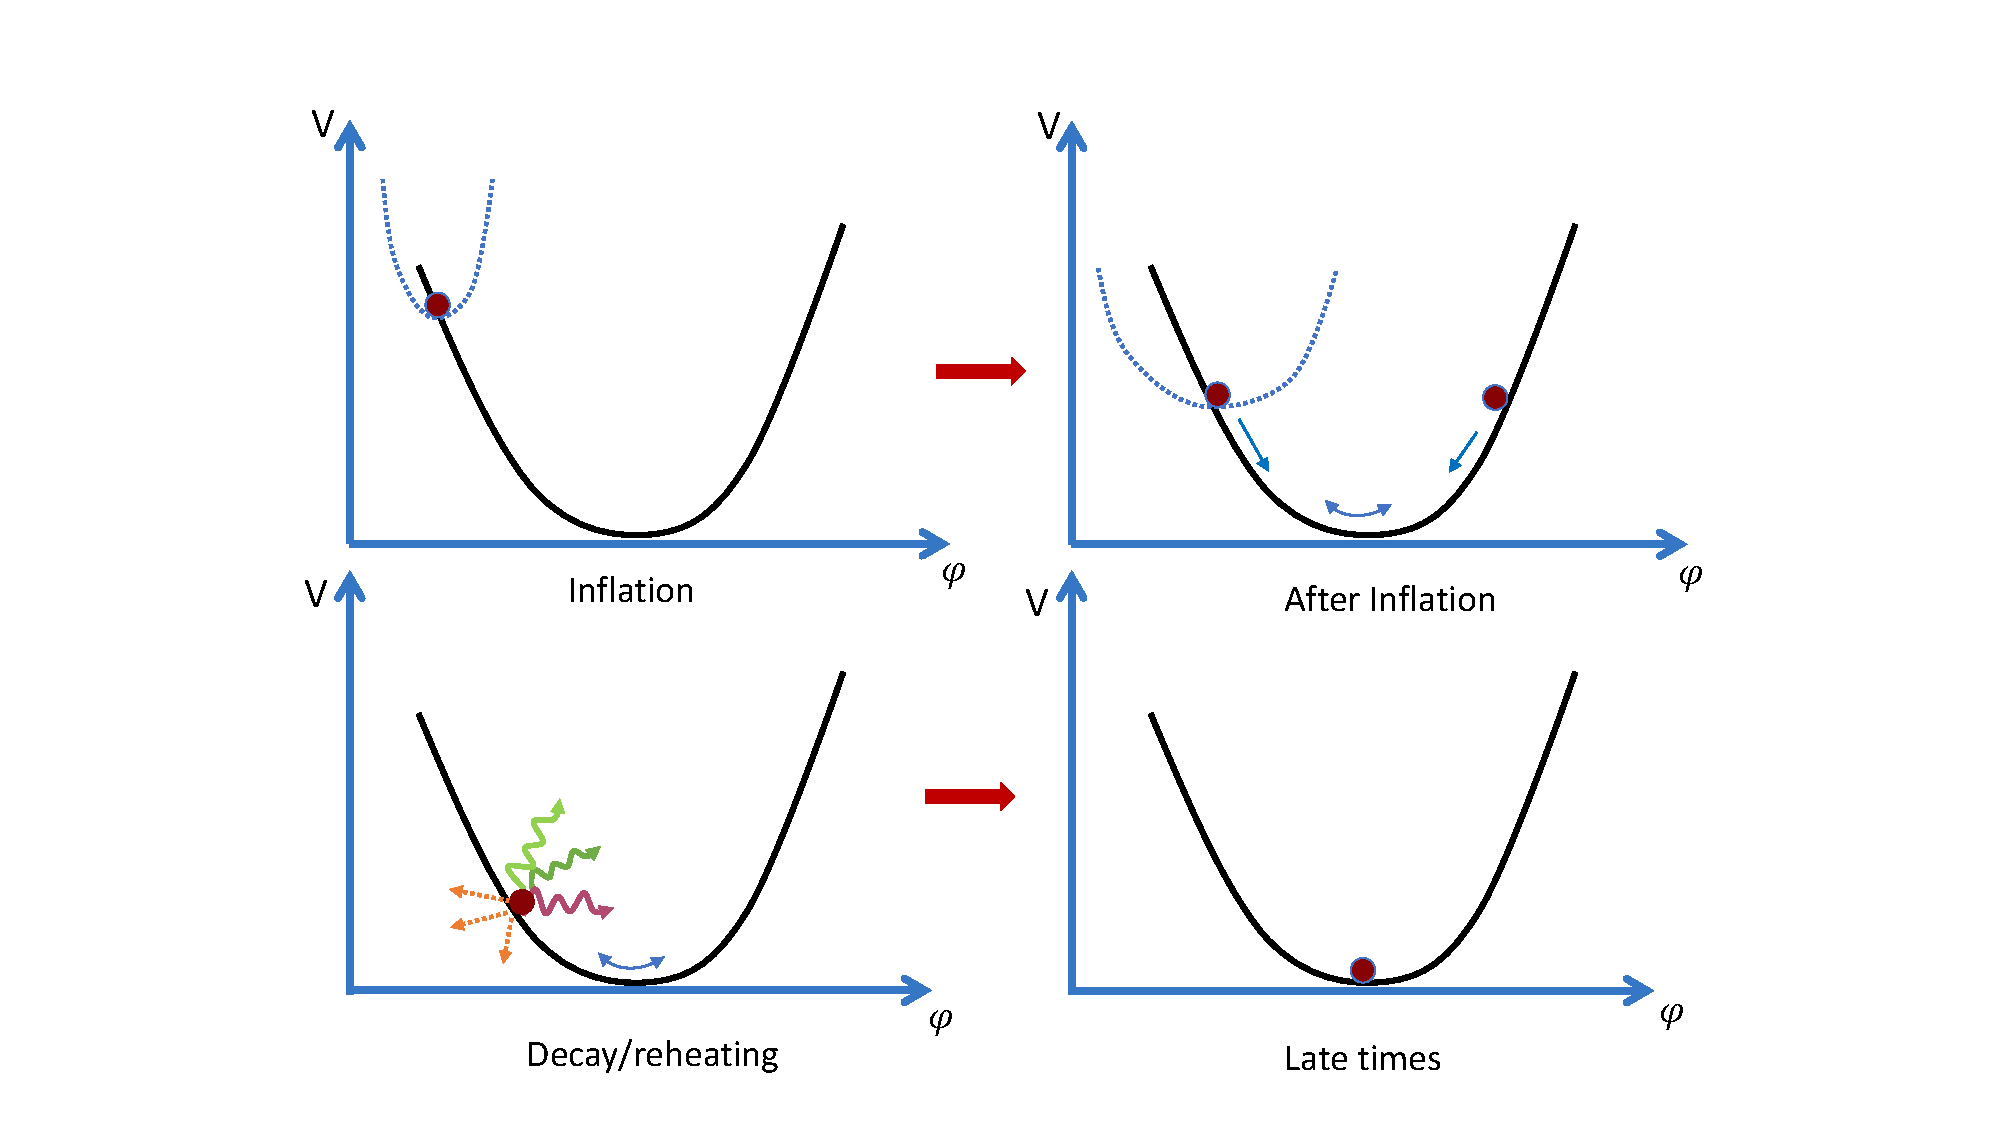
\includegraphics[width = 0.9\textwidth]{Sections/Figures/FigureModuliDomination.pdf} 
    \caption{Moduli domination. During inflation moduli fields which are not inflatons tend to be trapped at a point that does not correspond to their minimum. Only after inflation is finished do those moduli field start settling towards their minimum. Their coherent oscillations around this minimum come to dominate the energy density of the universe, behaving like matter domination, and particle production during this time is the source of reheating. This differs substantially from the standard picture of reheating from the inflaton right after inflation.}
    \label{fig:ModuliDomination}
\end{figure}




\subsection{Aspects of Moduli-Induced Reheating}

This epoch of moduli domination can affect various areas of early universe physics and
we now consider in more detail the implications of reheating driven by decays of moduli.

\subsubsection{The Cosmological Moduli Problem}

One of the best-known issues associated with moduli reheating is the \emph{cosmological moduli problem} (CMP) \cite{CoughlanRoss, hepph9308292, hepph9308325}. The $M_{\rm Pl}$-suppression in moduli interactions implies that they are long-lived. While the masses of moduli are model-dependent to some extent, in most cases these masses are comparable to the gravitino mass. When low-energy gravity-mediated supersymmetry is used to solve the hierarchy problem of the Standard Model, the soft terms are also normally comparable to the gravitino mass (note that for gauge-mediated models, $m_{3/2} \ll 1\, {\rm TeV}$, and this issue becomes more severe). For `generic' supergravity models, we then have
\begin{equation}
m_\phi \sim m_{3/2} \sim M_{\rm soft} \sim 1 \,{\rm TeV}\,,
\end{equation}
where $m_\phi$ denotes the modulus mass. For such mass scales, it
follows from Eq. (\ref{reheatmoduli}) that the resulting reheating temperature is $T_{\rm rh} \lesssim 1 \, {\rm MeV}$, insufficient for conventional nucleosynthesis. Generally, in any case where the lightest moduli have masses $m_\phi \lesssim 30\, \hbox{TeV}$, the period of moduli domination extends until a time period later than when Big Bang Nucleosynthesis (BBN) occurred. 
As observations of primordial element abundances make us highly confident that the standard picture of BBN is correct, such cosmologies are inconsistent with nature.

The above was first realised in the 1980s by Coughlan, Fischler, Kolb, Raby and Ross \cite{CoughlanRoss} for the supergravity Polonyi field and is the original cosmological moduli problem. It was subsequently re-emphasised and shown to be generic in the context of stringy scenarios of moduli stabilisation in \cite{hepph9308292, hepph9308325} and has existed since then as a standard reference point in discussions of string cosmology. The importance of this problem lies in its genericity: as long as moduli exist, they will tend to survive at low energies and tend to dominate the energy density of the universe. The original arguments relied on the assumption of low-energy supersymmetry to estimate their masses. However, the argument is more general than supersymmetry. Even if compactifications do not preserve supersymmetry, as long as the Kaluza-Klein scale is smaller than the Planck mass the moduli will survive at low energies. As moduli are the zero modes of Kaluza-Klein field, they only obtain masses through quantum effects. It is easy to estimate that their masses are at most of order $M_{KK}^2/M_{\rm Pl}$ \cite{Burgess:2010sy} which is much smaller than the KK and string scales as long as $M_{KK}<M_{\rm Pl}$.

The cosmological moduli problem is associated to the \emph{time} at which moduli decay, and through this, the Hubble scale (i.e. temperature) at which a conventional radiation-dominated Hot Big Bang is initiated. It may be useful here to distinguish here between a \emph{hard} cosmological moduli problem and a \emph{soft} cosmological moduli problem. 

The hard CMP is the requirement that $T_{\rm rh} > T_{\rm BBN}$: we \emph{know} that BBN occurred and so it is an absolute necessity that the reheat temperature is in excess of the temperatures required for BBN. There are several other aspects of physics we \emph{think} originated in the thermal Hot Big Bang, but where a precise answer is not known. Examples include mechanisms for baryogenesis and 
the origin of the dark matter relic abundance. Scenarios for these can require $T_{\rm rh} \gg T_{\rm BBN}$. As examples, scenarios of thermal leptogenesis can require $T_{\rm rh} \gtrsim 10^{11}\,{\rm GeV}$ \cite{Buchmuller:2005eh} whereas thermal freeze-out of WIMP dark matter tends to require $T_{\rm rh} \gtrsim m_{\rm DM}/20$, where $m_{\rm DM}$ is the dark matter mass. The soft CMP refers to the requirement that $T_{\rm rh}$ is sufficiently high to allow for all the other particle  physics, in addition to BBN, that we would like to occur in the Hot Big Bang. As the name suggests, this requirement is more nuanced and model-dependent, being tied to the actual physics used to generate (for example) the baryon asymmetry.

Since its original formulation, the importance of the CMP as a problem has waxed and waned. Most obviously, the `Problem' in the title originates from an assumption that supersymmetry would be present at TeV energy scales and would solve the hierarchy problem of the Standard Model. If low-energy supersymmetry is entirely absent -- or even if it simply ameliorates the hierarchy problem by appearing at 1000 TeV energy scales -- then the hard CMP loses its force. It is certainly true that, since the CMP was first proposed, the energy scales at which supersymmetry might plausibly be present have risen by an order of magnitude.

A further aspect is the development of explicit models of moduli stabilisation. The original CMP was formulated based on the properties of `generic' ${\cal N}=1$ 
supergravity scalar potentials. With the construction of actual scenarios of moduli stabilisation, it was realised that these `generic' expectations are often violated in actual models, which have additional structure compared to `generic' expectations. We give two examples.

The first example involves models based on non-perturbative stabilisation, where a gaugino condensate is balanced against either a constant term or another gaugino condensate. The standard examples of these are KKLT and racetrack models, as discussed in Sec.~\ref{ModuliSection}. In this case, there is a logarithmic enhancement in the masses of moduli relative to the gravitino mass, and also a logarithmic suppression in the mass of the soft terms relative to the gravitino mass \cite{hepth0411066, hepth0503216, hepph0702146}. More specifically
\begin{equation}
m_\phi \sim \ln \left( \frac{M_{\rm Pl}}{m_{3/2}} \right) m_{3/2} \sim \ln^2 \left( \frac{M_{\rm Pl}}{m_{3/2}} \right) M_{\rm soft}\,.
\label{kkltsoft}
\end{equation}
This implies that soft terms at $\sim 1 \, \rm{TeV}$ would actually be accompanied by moduli masses at 1000 TeV, greatly ameliorating the cosmological moduli problem.

The second example involves models which start with a no-scale structure (of which LVS is the principal example). At leading order (i.e. with exact no-scale as in GKP \cite{Giddings:2001yu}) a modulus remains massless despite the presence of both a finite gravitino mass and broken supersymmetry. In the full vacuum, this structure still survives 
approximately, with a modulus parametrically lighter than the gravitino mass:
\begin{equation}
m_\phi \ll m_{3/2}\,.
\label{noscalemass}
\end{equation}
The form and scale of the soft terms depends on the realisation of the Standard Model and the degree of sequestering present. Two possible scenarios have been identified \cite{Blumenhagen:2009gk, Aparicio:2014wxa, Reece:2015qbf}, building on earlier analyses of LVS soft terms in \cite{hepth0605141, hepth0609180, hepth0610129}. These lead to either  
\begin{equation}
m_{3/2} \sim \frac{M_{\rm Pl}}{\mathcal{V}} \gg m_\phi \sim M_{\rm soft} \sim \frac{M_{\rm Pl}}{\mathcal{V}^{3/2}}\,,
\label{lvssoft1}
\end{equation}
or
\begin{equation}
m_{3/2} \sim \frac{M_{\rm Pl}}{\mathcal{V}} \gg m_\phi  \sim \frac{M_{\rm Pl}}{\mathcal{V}^{3/2}} \gg M_{\rm soft} \sim \frac{M_{\rm Pl}}{\mathcal{V}^2}\,.
\label{lvssoft2}
\end{equation}
Irrespective of which case is realised, what Eqs. (\ref{kkltsoft}), (\ref{lvssoft1}) and (\ref{lvssoft2}) have in common is a pattern of masses very different to that assumed in the `generic' CMP.

Despite these results, and the general softening of the CMP in the absence of a discovery of weak scale supersymmetry, it persists as a question that must be addressed in all stringy cosmologies. Even if the hard CMP is not a problem as such, it is also a reminder that stringy cosmologies are expected to have lower reheating scales than in more conventional field theory models of the early universe.

\subsubsection{Dark Radiation Constraints on Moduli Decays}

The cosmological moduli problem is primarily associated with the \emph{time} at which moduli decay, and the danger that the transition to radiation domination occurs too late for conventional BBN epoch.

Other potential problems (or opportunities!) are associated to the decay products and branching ratios of moduli. As with the CMP, these problems can be formulated both  `generically' in terms of supergravity models without special structure in the couplings, and then refined in terms of the precise structures that arise within particular string compactifications. As with the CMP, the origin of all such problems is the requirement that reheating cannot lead to a universe that is significantly different than a radiation-dominated Hot Big Bang, in which almost all energy is contained in Standard Model degrees of freedom.

In particular, if significant amounts of energy density are injected into degrees of freedom that are decoupled from the Standard Model, this may lead to significant cosmological tensions. The simplest example of this is an over-production of \emph{dark radiation} -- a possible additional relativistic contribution to the energy density which is decoupled from the Standard Model degrees of freedom. While today, after ten billion years of matter and dark energy domination, such radiation would only contribute negligibly to the dynamics of the universe, in earlier epochs such radiation would significantly affect the expansion history. 

From observations of the CMB, we know that the early universe bounds the amount of additional `dark' radiation that can contribute to the energy density. This is conventionally expressed in terms of a bound on the number of effective neutrino species; this reflects the fact that, after they decouple, the neutrinos free-stream as relativistic particles decoupled from the other Standard Model degrees of freedom, and so behave (effectively) as dark radiation.
The magnitude of this limit can be expressed as \cite{Planck:2018vyg}:
\begin{equation}
\setlength\fboxsep{0.25cm}
\setlength\fboxrule{0.4pt}
\boxed{
\Delta N_{\rm eff} \lesssim 0.2\,.
}
\end{equation}
Here $N_{\rm eff}$ is the effective number of `extra' neutrino species beyond those of the Standard Model.

String compactifications contain many particles which could in principle constitute dark radiation, as they are both light and very weakly coupled to the Standard Model. One example is gauge bosons of unbroken dark sector gauge groups. These can arise either as hidden $U(1)$s present on `distant' branes within D-brane constructions or alternatively from $n$-form potentials reduced on internal $(n-1)$-cycles (e.g. $A^i_\mu = \int_{\Sigma_2^i} C_3$). Another type of particle with light and `protected' masses are chiral fermions belonging to matter sectors decoupled from the Standard Model. In models of branes at singularities, these can arise from matter originating on branes located at distant singularities. Here, the chirality protects the mass of the particles while the geometrical separation ensures the weakness of couplings to the Standard Model and ensures that such particles will not thermalise with Standard Model degrees of freedom.

However, in terms of dark radiation candidates within string theory, arguably the most appealing and universal particle candidates are axions or axion-like particles (ALPs) \cite{Svrcek:2006yi, Arvanitaki:2009fg, Cicoli:2012sz, Demirtas:2018akl}. Axions are $U(1)$-valued scalars: instead of the real line, they take values on a circle. They have a perturbative shift symmetry $a_i \to a_i + 2 \pi f_a$, which ensures that the potential remains flat to all orders in perturbation theory. Here $f_a$ is the \emph{axion decay constant} which specifies the radius of the $U(1)$ circle and also governs the strengths of axion-matter couplings. As non-perturbative corrections are exponentially suppressed, it is natural (depending on the precise details of the compactifications) for ALPs to remain effectively massless, and in particular sufficiently light so as to be a good candidate for dark radiation. The shift symmetry also implies that axions must couple via derivative interactions, which implies that their interactions with the Standard Model are suppressed by their decay constant $f_a \gg 1\, \rm{TeV}$. For all these reasons, energetic relativistic axions produced in the early universe are likely to persist as a relativistic background until the present day (forming what has been called a Cosmic Axion Background \cite{13053603, 210109287}).

We aim to formulate the generic problem succinctly. In string theory, reheating tends to be driven by moduli with gravitational-strength couplings. Certain moduli (for example, the overall volume modulus or the dilaton modulus) tend to couple to all sectors of the theory in a broadly democratic fashion. However, as there could easily be hundreds of hidden-sector particles, 
democratic decays would likely result in too much energy going into axions or other hidden sector modes. The decay modes 
\begin{equation}
\phi \to {\rm hidden}\,,
\end{equation} 
may produce dark radiation at a level far above the observable limits. As moduli-dominated reheating is generic in string theory, this constitutes a generic problem (or opportunity!) for string models of reheating. 

This problem of \emph{excessive dark radiation} is generic within string compactifications. If reheating originates from gravitationally-coupled sectors, it is hard to see why the fractional decay rate to non-Standard Model light hidden sectors should be close to zero: what makes the Standard Model sector special and preferred?

To formulate this problem more precisely, and move beyond generic statements, requires actual vacua in which we can determine the longest-lived modulus, its mass, its couplings and its decay modes. Although the `visible sector' in principle requires the actual Standard Model, even without a full Standard Model realisation in a compactification, toy proxies for a Standard Model can be used (for example, a D3-brane probing a Calabi-Yau singularity or a stack of D7-branes wrapping a divisor in the geometric regime) to allow for the calculation of decay modes to a `quasi-visible' sector.

As a consequence of its parametric scale separation, the Large Volume Scenario provides a clean environment in which the lightest modulus and its couplings can be determined. It is not surprising then, that in the context of LVS, this problem has been formulated especially sharply, starting originally with \cite{Cicoli:2012aq, 12083563} and then developed further on in 
\cite{12113755, 13041804, 13054128, Allahverdi:2014ppa, Angus:2014bia, 14036810, Cicoli:2015bpq, Cicoli:2018cgu, 210713383, Cicoli:2022fzy, Cicoli:2022uqa}. 

Focusing on LVS Calabi-Yau models where the overall volume is controlled by a single modulus, the lightest modulus is the overall volume modulus, which allows for a precise computation of the couplings and decay modes. These couplings are set by the relevant K\"ahler and superpotential terms. The superpotential terms drop out, as K\"ahler moduli such as the overall volume only appear in the superpotential non-perturbatively. The dependence of matter kinetic terms on the volume direction itself is given by 
\begin{equation}
K_{T\overline{T}} \propto \frac{1}{\mathcal{V}^{2/3}}\,.
\label{matterkahlermetric}
\end{equation}
This follows from the modulus K\"ahler potential $K = - 2 \ln \mathcal{V}$ and the requirement that the physical Yukawa couplings in local models are determined locally and so must be independent (at tree-level) of the overall volume \cite{hepth0609180}. The self-couplings of the volume multiplet can be found from the K\"ahler potential
\begin{equation}
K = - 3 \ln \left( T + \overline{T} \right),
\end{equation}
where $T$ is the superfield containing the volume modulus.
This is equivalent to $K = - 2 \ln \mathcal{V}$ when we restrict to only the overall volume mode. The resulting kinetic terms are
\begin{equation}
\mathcal{L}_{\rm kin} = \frac{3}{4 \tau_b^2} \partial_{\mu} \tau_b \partial^{\mu} \tau_b + \frac{3}{4 \tau_b^2} \partial_{\mu} a\, \partial^{\mu} a\,.
\label{Lvol}
\end{equation}
From Eq. (\ref{Lvol}) we can read off the couplings of the volume modulus to its own axion.

Assuming an MSSM-like local matter sector and no additional dark sectors, it was found in \cite{Cicoli:2012aq, 12083563} that there are \emph{two} dominant decay modes: the decay $\phi \to aa$ of the volume to the volume axion, and the decay $\phi \to H_1 H_2$ which proceeds via the Giudice-Masiero $\mu$-term. The coupling to the axion is universal and after canonical normalisation takes the form \cite{Cicoli:2012aq, 12083563}
\begin{equation}
\mathcal{L} = \frac34 \exp \left( -2 \sqrt{\frac23} \phi \right) \partial_{\mu} a \,\partial^{\mu} a\,,
\end{equation}
which gives a decay width
\begin{equation}
\setlength\fboxsep{0.25cm}
\setlength\fboxrule{0.4pt}
\boxed{
\Gamma_{\phi \to aa} = \frac{1}{48 \pi} \frac{m_\phi^3}{M_{\rm Pl}^2}\,.
}
\label{axionwidth}
\end{equation}
This axionic contribution to dark radiation is universal and unavoidable, as the volume axion is always present in the compactification, and at large volumes the couplings are entirely set by the tree-level K\"ahler potential. As well as these decays to the volume axion, the volume modulus can also decay to other light open- or closed-string axions present in the compactification \cite{210713383, Cicoli:2022uqa}.

Interestingly, all matter decay modes \emph{except} the one proceeding via a Giudice-Masiero term 
\begin{equation}
K = \dots + \left( \frac{Z H_u H_d}{\left( T_b + \overline{T}_b \right)} + {\rm c.c.} \right) + \dots 
\end{equation}
are  suppressed by an $\left(M_{\rm soft}/m_\phi\right)^2\ll 1$ factor, as the K\"ahler potential of Eq. (\ref{matterkahlermetric}) leads to a coupling
\begin{equation}
\phi ( {Q} \nabla^2 Q + Q \nabla^2 \bar{Q})\,,
\end{equation}
which is suppressed on-shell by a relative factor $\left(M_{\rm soft}/m_\phi\right)^2$ compared to modes like Eq. (\ref{axionwidth}). Note that in models where the visible sector is sequestered from the sources of supersymmetry breaking, also the decay of the volume mode into MSSM gauge bosons is suppressed since the tree-level gauge kinetic function is set by the dilaton. Meanwhile, the Giudice-Masiero term gives a decay width
\begin{equation}
\setlength\fboxsep{0.25cm}
\setlength\fboxrule{0.4pt}
\boxed{
\Gamma_{\phi \to H_u H_d} = \frac{2 Z^2}{48 \pi} \frac{m_\phi^3}{M_{\rm Pl}^2}\,,
}
\end{equation}
very similar to the axion decay width of Eq. (\ref{axionwidth}). 

Although some aspects are model-dependent (for example, the branching ratio to the Standard Model depends on the undetermined constant $Z$ and would be enhanced for models with extended Higgs sectors), this calculation illustrates the way in which moduli-dominated reheating is expected to produce dark radiation. Depending on perspective, this can be viewed either as a problem or an opportunity for such models. 

Another contribution to the volume mode decay into two Standard Model Higgs degrees of freedom $h$ comes from moduli-dependent loop corrections to the Higgs mass \cite{Cicoli:2022fzy}:
\begin{equation}
m_h^2 = M_{\rm soft}^2 \left[c_0 + c_{\rm loop} \ln\left(\frac{M_{\rm KK}}{m_{3/2}}\right)\right] 
\end{equation}
which, using $M_{\rm KK}\sim M_{\rm Pl}/\mathcal{V}^{2/3}$, induces the following couplings:
\begin{equation}
\mathcal{L}\supset -\sqrt{\frac32} \frac{m_h^2}{M_{\rm Pl}}\,\phi \,h^2 + \frac{c_{\rm loop}}{4}\sqrt{\frac32} \frac{M_{\rm soft}^2}{M_{\rm Pl}}\,\phi \,h^2\,.
\label{LoopCoupl}
\end{equation}
Clearly, the first coupling is irrelevant since it is suppressed by the Higgs mass. However the second coupling would give rise to a decay width that scales as 
\begin{equation}
\Gamma_{\phi \to hh} \sim \left(\frac{c_{\rm loop}}{Z}\right)^2 \left(\frac{M_{\rm soft}}{m_\phi}\right)^4\,\Gamma_{\phi \to H_u H_d}\,.
\end{equation}
For models without sequestering (which requires the Higgs mass to be fine-tuned to be much lighter than its `natural' value), $M_{\rm soft}\sim m_{3/2}\gg m_\phi$, $\Gamma_{\phi \to hh}$ dominates over $\Gamma_{\phi \to H_u H_d}$ and $\Gamma_{\phi \to aa}$, guaranteeing the absence of any dark radiation production. On the other hand, in sequestered models, $M_{\rm soft}\lesssim m_\phi$, implying that $\Gamma_{\phi \to hh}$ is subdominant with respect to $\Gamma_{\phi \to H_u H_d}$.

In a phenomenologically realistic scenario, it is obviously critical that the amount of dark radiation produced does not exceed the observational bounds. One approach to achieving this is to enhance the modulus couplings to the visible sector. For example, in sequestered models, one may assume that $Z \gg 1$ or that actual BSM physics involves a large number of Higgs sectors which enhances the visible sector branching ratio purely on multiplicity grounds. 

Although it is fair to describe LVS as the most developed scenario for precise studies of reheating and dark radiation production, similar questions of dark radiation production have also been studied for other scenarios of moduli-stabilisation, for example see \cite{ 13047987, 14072501, 150207746, 151207907,  190603025, 210803317, Baer:2023bbn}.

Our discussion has mostly treated the existence of dark radiation from moduli decay as a problem to be expunged. However, one can also regard it as an opportunity to be seized. The electromagnetic interactions of photons imply that the photon surface of last scattering is the CMB, which dates from a time 380,000 years after the Big Bang. For axion-like particles, the similar surface of last scattering extends deep into the primordial epoch of the universe, reaching far earlier than the epoch of BBN. Indeed, one would expect that a typical axion-like particle produced from modulus decay would propagate to the present day without interacting once. If it were possible to detect these particles, they would give a direct probe of the universe at an exceedingly early period. Such a surviving background of relativistic dark radiation cosmic axions was called a `Cosmic Axion Background' in \cite{13053603} and its phenomenology and detection possibilities studied in 
 \cite{13066518, 13104464, 13123947, 14065188, 14072501, 14114172, 150605334, 160208433, 210703420, Bhattacharya:2020zap, Banerjee:2022era}.

\subsubsection{Moduli-Induced Gravitino Problems}

As well as decays to axions or other massless particles, another potentially problematic channel for moduli decays is the decay mode to gravitini. If the lightest modulus has a mass $m_\phi > 2 m_{3/2}$, it can decay via the process $\phi \to 2 \psi_{3/2}$. If the modulus is gravitationally coupled and related to the superfield which broke supersymmetry (and thus generates the two spin-$\frac12$ components of the gravitino in the super-Higgs effect), we expect it couple to the gravitino modes and so have a notable branching ratio to gravitini. 

This is true in both KKLT and racetrack stabilisation. For the case of the hierarchically small gravitino masses required to address
the electroweak hierarchy problem,
\begin{equation}
m_\phi \sim \ln \left( \frac{M_{\rm Pl}}{m_{3/2}} \right) m_{3/2} \gg m_{3/2}\,,
\end{equation}
and so the gravitino can be treated as effectively massless compared to the modulus (as $m_{3/2} \sim m_\phi/30$). However, it is not true for LVS, where the inverse hierarchy $m_\phi \ll m_{3/2}$ applies.

The dangers of this decay channel were emphasised in \cite{hepph0602061, hepph0602081}, where it was dubbed the \emph{moduli-induced gravitino problem}. The dangers arise as the gravitini are long-lived and such long-lived gravitini can cause several problems. In particular, they can interfere with BBN if they live long enough so that they decay after the start of BBN with a late injection of energy (effectively reintroducing the modulus problem). Another problem can arise with the dark matter abundance. If the gravitini are stable, as in gauge-mediated scenarios, then the decay can result in over-production of dark matter. However, even if unstable then the decay can result in an overproduction of the neutralino LSP.

Building on the original work, further studies of the moduli-induced gravitino problem have been performed in \cite{hepph0603265, hepph0604140, hepph0604132, hepph0605297, hepph0607170, hepph0701042, hepph0703319, Heckman:2008jy, 09043773, 09082430, 12092583, 12104077, 13110052, 150402040, 160308399, 220106633}.

\subsubsection{Post-inflationary History and Predictions from Inflation}

As discussed in chapter \ref{SecCO}, in inflation the predictions for the spectral tilt and the tensor-to-scalar ratio are determined by the number of e-foldings $N_e$ between horizon exit of the CMB modes and the end of inflation. The quantity $N_e$ is determined by the so called `matching equation' which is the condition obtained by tracking the evolution of the energy density of the universe from the time of horizon exit of the CMB modes to the present times (see e.g. \cite{Planck:2013jfk}). Thus, inflationary predictions are sensitive to the post-inflationary history of the universe. As we have seen, in string models the presence of light moduli generically leads to a non-standard post-inflationary history involving epochs of moduli domination. This, in turn, affects the precise predictions and is crucial for obtaining the best fit regions for string inflationary models \cite{Easther:2013nga, Dutta:2014tya, Bhattacharya:2017ysa, Cicoli:2020bao, Bhattacharya:2020gnk, Neves:2020anh}. The analysis of \cite{Bhattacharya:2017ysa, Bhattacharya:2020gnk} integrates the CosmoMC analysis with Modechord \cite{Handley:2015fda} allowing for extraction of the best fit regions in the parameter space.



\subsubsection{Finite-temperature Corrections and Decompactification}

Reheating at the immediate end of inflation can produce an initial epoch of radiation domination with several particles in thermal equilibrium. 
Although this may subsequently be diluted by moduli,
this generates finite-temperature corrections which in 4-dimensional string models can be a dangerous source of decompactification, see e.g \cite{Buchmuller:2004xr, Buchmuller:2004tz, Danos:2008pv, Anguelova:2009ht, DiMarco:2019czi, Gallego:2020vbe,Alam:2022rtt}. This can be seen from the fact that thermal loops yield a moduli-dependent contribution to the scalar potential of the form (at 1- and 2-loop order):
\begin{equation}
\setlength\fboxsep{0.25cm}
\setlength\fboxrule{0.4pt}
\boxed{
V_T \sim T^4 g^2 + T^2 M_{\rm soft}^2\,,
\label{VT}
}
\end{equation}
where $g^2\sim \tau_{\rm SM}^{-1}$ is the Standard Model coupling set by the modulus supporting the stack of branes which reproduce the visible sector, and $M_{\rm soft}\lesssim m_{3/2}$ is the mass of the supersymmetric particles running in the loop (we ignored ordinary matter since it would give rise to a subdominant contribution). 

As we have already seen, the KKLT potential scales as $V_{\rm KKLT}\sim m_{3/2}^2 M_{\rm Pl}^2$ while the LVS potential scales as $V_{\rm LVS}\sim m_{3/2}^3 M_{\rm Pl}$. Given that $M_{\rm soft}\lesssim m_{3/2}$ and $T< M_{\rm Pl}$, the second term in (\ref{VT}) is always a small correction to the KKLT potential. This is true also in the LVS case since $T < M_{\rm KK} \sim M_{\rm Pl}/\mathcal{V}^{2/3}$ implies $T^2 M_{\rm soft}^2 < M_{\rm KK}^2 m_{3/2}^2 \sim M_{\rm Pl}^4/\mathcal{V}^{10/3} \ll V_{\rm LVS} \sim M_{\rm Pl}^4/\mathcal{V}^3$ for $\mathcal{V}\gg 1$. Hence the only dangerous term in (\ref{VT}) is the one proportional to $T^4$ which would cause a runaway towards decompactification unless $T^4 g^2$ is subdominant with respect to the zero-temperature moduli potential. This problem can be avoided if 
the initial reheating temperature is below a maximal temperature given in KKLT by \cite{Buchmuller:2004tz}: 
\begin{equation}
T_{\rm rh}<T_{\rm max}\sim \sqrt{m_{3/2} M_{\rm Pl}}\sim 10^{11}\,{\rm GeV}\quad\text{for}\quad m_{3/2}\sim 10\,{\rm TeV}
\end{equation}
and in LVS by \cite{Anguelova:2009ht}:
\begin{equation}
T_{\rm rh}<T_{\rm max}\sim \left(m_{3/2}^3 M_{\rm Pl}\right)^{1/4}\sim 10^8\,{\rm GeV}\quad\text{for}\quad m_{3/2}\sim 10\,{\rm TeV}\,.
\end{equation}

\subsubsection{Baryogenesis and Moduli-Domination}

As we have seen, 4-dimensional string models are characterised by late-time epochs of moduli domination which end when the moduli decay, leading to a reheating temperature of order $T_{\rm rh}\simeq 0.1\,m_\phi\sqrt{m_\phi/M_{\rm Pl}}$. The actual value of $T_{\rm rh}$ clearly depends on the lightest modulus mass $m_\phi$, which in string models is correlated with the scale of supersymmetry breaking. As an illustrative example, consider LVS models with sequestered supersymmetry breaking which can lead to TeV-scale supersymmetry without a cosmological moduli problem. In this case $m_\phi \sim M_{\rm soft}^{3/4} M_{\rm Pl}^{1/4}$. For $M_{\rm soft}\sim 1$ TeV, we obtain $m_\phi \sim\mathcal{O}(10^7)$ GeV which, in turn, leads to $T_{\rm rh}\sim \mathcal{O}(1-10)$ GeV. This reheating temperature is clearly too low to allow for standard scenarios of baryogenesis like thermal leptogenesis or EW baryogenesis which require higher reheating temperatures (and so much larger moduli masses, incompatible with any form of low-energy supersymmetry). 

If we require (relatively) low-energy supersymmetry, a reheating temperature around $T_{\rm rh}\sim \mathcal{O}(1-10)$ GeV necessitates a non-thermal mechanism for baryogenesis. One interesting option is given by Affleck-Dine baryogenesis \cite{Affleck:1984fy} that exploits MSSM D-flat directions which carry a net baryon number. If lifted by supersymmetry breaking effects, they can acquire a non-zero VEV during inflation. After inflation, they first oscillate around the minimum and then decay into fermions generating baryon asymmetry. Interestingly ref. \cite{Allahverdi:2016yws} has shown that in K\"ahler moduli inflation inflaton-dependent F-terms can induce tachyonic masses during inflation for these MSSM D-flat directions, creating the right initial conditions for Affleck-Dine baryogenesis. However, this mechanism has the problem of generating (in general) too much baryon asymmetry. Nevertheless, this can be avoided in string models where the initial baryon asymmetry is diluted by the decay of the lightest modulus which gives \cite{Kane:2011ih}:
\begin{equation}
\frac{n_B}{s} \simeq \frac{|A|}{m_\phi}\frac{T_{\rm rh}}{m_\phi}\left(\frac{\phi_0}{M_{\rm Pl}}\right)^2\,,
\end{equation}
where $A$ is the soft trilinear $A$-term, $\phi_0$ the initial modulus displacement and $n_b/s$ the baryon-to-entropy ratio. Interestingly, the values $|A|\sim 1$ TeV, $m_\phi\sim 10^6$ GeV, $T_{\rm rh}\sim 1$ GeV and $\phi_0\sim \mathcal{O}(0.1-1)\,M_{\rm Pl}$, can naturally reproduce the observed baryon-to-entropy ratio $n_B/s\sim 10^{-10}$.  Affleck-Dine baryogenesis after (string) axion inflation was studied in \cite{Akita:2017ecc}, where it was found the axion oscillations could produce sufficient baryon asymmetry just after inflation even without a soft-supersymmetry breaking $A$-term.

\subsection{Non-standard cosmologies from D-branes}
\label{ssec:DST} 

From our discussion so far, it is clear that string theory cosmology models strongly motivate non-standard cosmological evolution. In particular, the epoch between the end of inflation and the onset of BBN remains highly unconstrained by current observations. Such non-standard evolution can be driven by the scalar fields in the theory as discussed above (see Fig.~\ref{fig:AlternativeHistory}).

Besides kination and moduli domination, a different scenario arises when D-branes are present. For D-branes moving in the internal compact space, the scalar field(s) associated to the open string representing, e.g.~the radial position of a D-brane along a warped throat, couples {\em disformally} to  matter living on such a brane \cite{Koivisto:2013fta}. Indeed, the induced metric on the brane takes the form $\tilde g_{\mu\nu} = C(\phi) g_{\mu\nu} + D(\phi) \partial_\mu\phi \partial_\nu\phi$, which is a particular case of the more general relation between two metrics in scalar-tensor theories introduced by Bekenstein in \cite{Bekenstein:1992pj}. This non-trivial coupling between matter and the scalar field can change the cosmological expansion rate, $\tilde H$ in the early evolution of the universe with interesting and potentially testable implications\footnote{See \cite{Allahverdi:2020bys} for a review on implications of non-standard cosmologies.}. Interestingly, for a `pure disformal' modification of the expansion rate, which arises for $C=1$, $D=D_0=$const.~from (stacks of) D-branes moving in the internal space in the early universe, the modified expansion rate can change the standard prediction for the production of thermal dark matter, giving earlier freeze-out temperatures and larger cross-sections compared to the standard case  \cite{Dutta:2016htz,Dutta:2017fcn}. 
Moreover, such an early period of D-brane scalar-tensor domination may be tested by its effect on the stochastic primordial gravitational wave background as shown in \cite{Chowdhury:2022gdc}. 
Due to non-standard cosmological expansion, the amplitude of the PGW spectrum can be enhanced over a wide range of frequencies covering various sensitivity ranges of future GW experiments such as LISA \cite{amaroseoane2017laser}, DECIGO \cite{Seto:2001qf}, and the Einstein Telescope \cite{Maggiore:2019uih}. Specifically, a disformally dominated epoch is characterised by a peaked spectrum with a {\em broken power-law} profile, with slopes that depend on the scalar-tensor theory considered \cite{Chowdhury:2022gdc} (see Fig.~\ref{Fig:DisformalGW}).  Moreover, if the scalar potential for the D-brane scalar field  satisfies suitable conditions, this scalar field can naturally source an early period of {\em early dark energy} \cite{Chowdhury:2023} (see sec.~\ref{subs:EDE}). Disformal D-brane scalar tensor theories are based on symmetries appearing in D-brane models with  interesting and potentially testable phenomenological implications. However, to fully explore their cosmological implications, it remains to embed  these scenarios into fully developed string constructions with moduli stabilisation. 

\begin{figure}[H]
\begin{center}
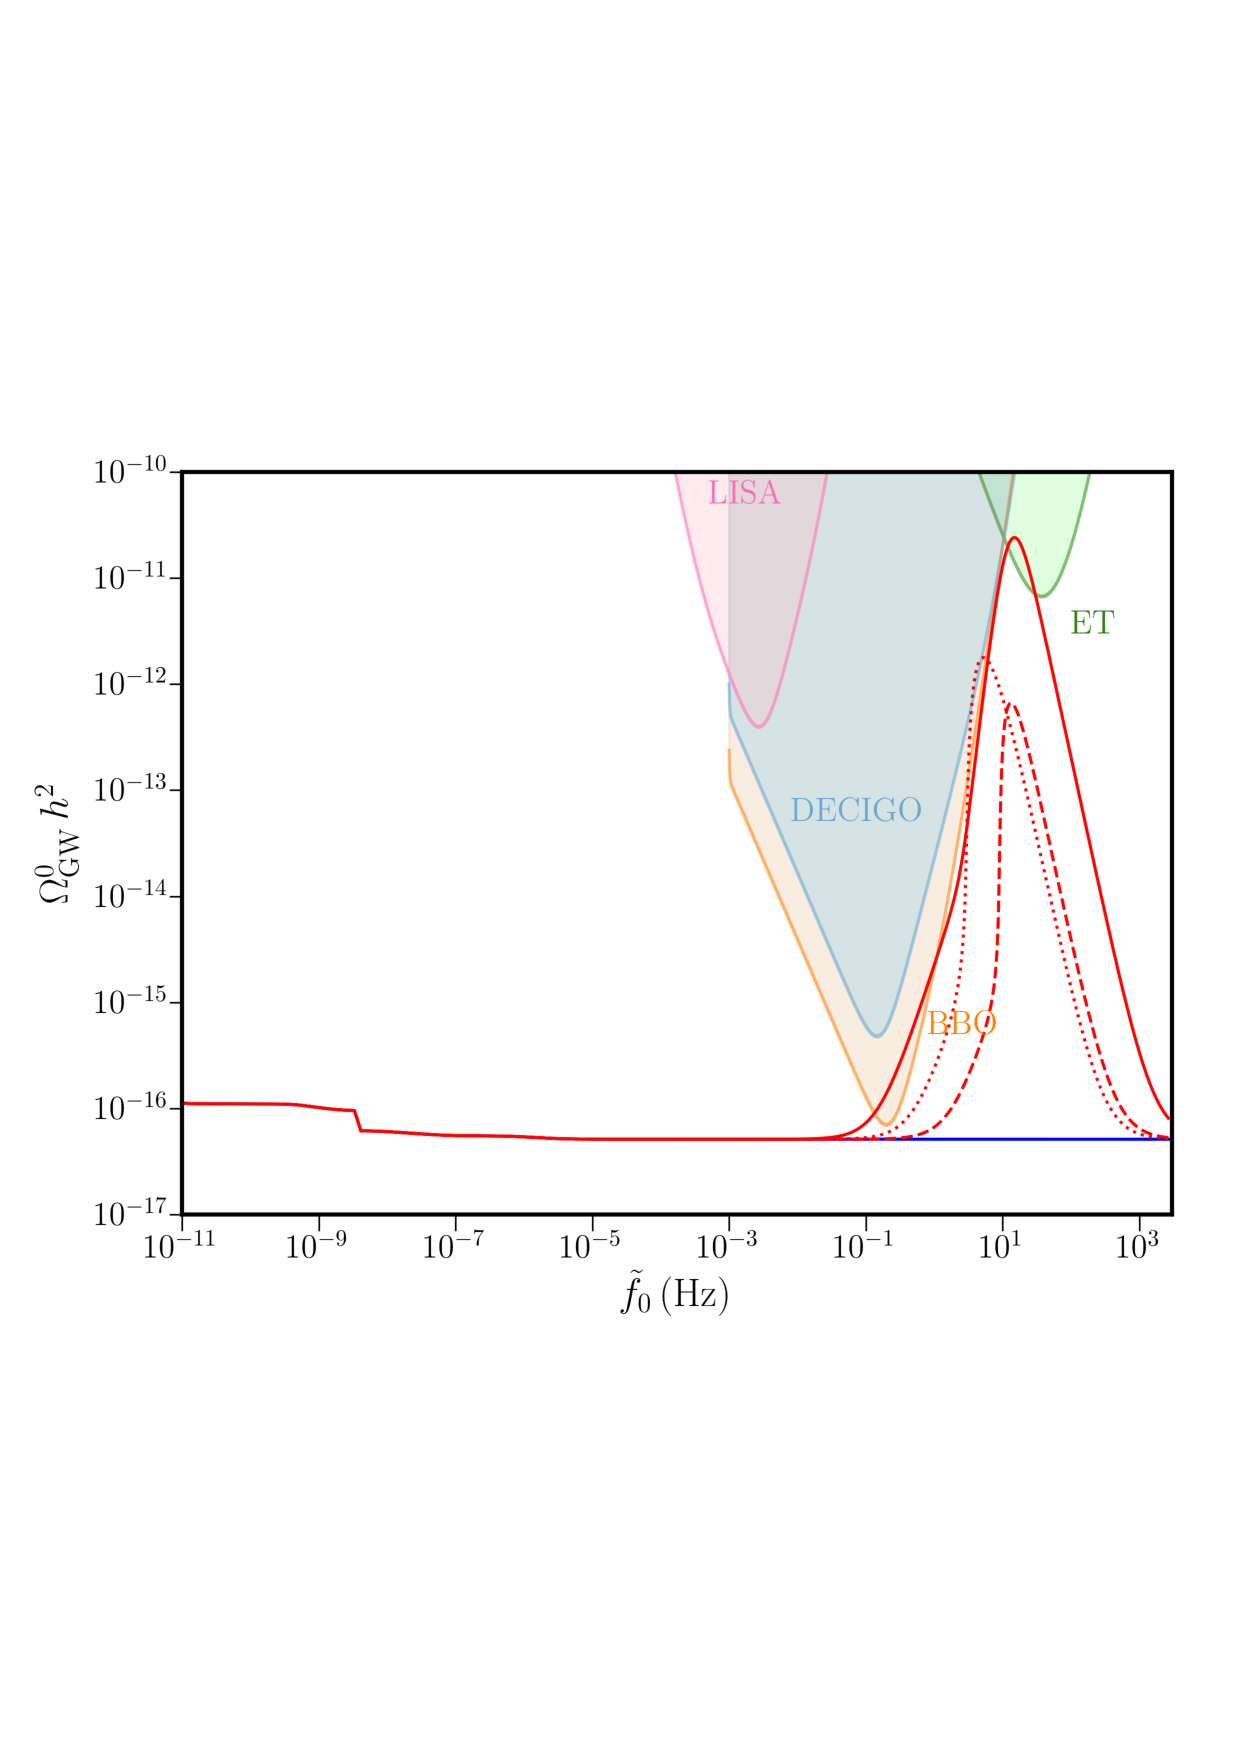
\includegraphics[width=10.00cm]{Sections/Figures/Disformal_GW.pdf}
\end{center}
\vskip -95pt
\caption{Gravitational wave spectrum for purely disformal D-brane scenarios with $C=1$, $D=D_0=4.822\times 10^{-37}{\rm GeV}^{-4}$, solid line. The vertical line indicates the frequency corresponding to the initial temperature ($\tilde T_i=10^{11}\,{\rm GeV}$). Figure taken from \cite{Chowdhury:2022gdc}, see this reference for further details.  (The dashed and dotted lines correspond to phenomenological cases discussed in \cite{Chowdhury:2022gdc}.)
}\label{Fig:DisformalGW}
\end{figure}




\subsection{Non-thermal Dark Matter from String Theory}

Post-inflationary eras of matter domination driven by late-time decaying string moduli have strong effects on dark matter. We briefly discuss here how moduli domination can modify the standard picture of the two most promising scenarios for dark matter: TeV-scale WIMPs and the QCD axion. We also comment on the possibility to realise fuzzy dark matter from string theory using ultra-light axions. Moreover we show how, in a given class of models, the underlying UV correlations between different aspects of string phenomenology can constrain the nature of dark matter. Finally we briefly comment on the string-inspired idea of dynamical dark matter.

\subsubsection{Non-thermal WIMPs}

Thermal WIMPs are arguably the most developed and best studied candidates for cold dark matter. In the standard paradigm they are assumed to be in thermal equilibrium in the early universe after inflation. Subsequently, dark matter drops out of thermal equilibrium and its abundance freezes out at a temperature of order $T_{\rm f} \sim m_{\rm DM}/20 \gtrsim 10$ GeV as annihilation becomes inefficient. This mechanism, even if it has been named the `WIMP miracle', requires a very specific annihilation cross section. For example, in the Minimal Supersymmetric Standard Model (MSSM), neutralino dark matter candidates typically give too much (for Bino-like neutralinos) or too little (for Higgsino/Wino-like neutralinos) relic density. 

However, from the string theory point of view, many standard thermal dark matter scenarios seem very hard to achieve since the generic late-time decay of long-lived moduli typically erases any previously produced dark matter relic density. Dark matter is instead 
produced non-thermally from the decay of the lightest modulus at $T_{\rm rh}$ \cite{Moroi:1999zb, Acharya:2008bk, Acharya:2009zt, Allahverdi:2013noa, 14091222, Allahverdi:2014ppa, Aparicio:2015sda, 150205406, 150804144, 151106768, Aparicio:2016qqb, Allahverdi:2018iod, Allahverdi:2020uax, 220106633, Cicoli:2022uqa}. The requirement to avoid any cosmological moduli problem and to obtain TeV-scale supersymmetry, typically yields stringy scenarios with $T_{\rm BBN} \sim \mathcal{O}(1)\,{\rm MeV} < T_{\rm rh}\sim \mathcal{O}(1)\,{\rm GeV} < T_{\rm f}\sim\mathcal{O}(10-100)\,{\rm GeV}$. 

Interestingly, non-thermal dark matter scenarios vastly enlarge the parameter space of particle physics models since the presence of an extra parameter, $T_{\rm rh}$, in the determination of the dark matter relic abundance, can allow portions of the parameter space which would be ruled out in the standard thermal case. Let us now analyse this point in more detail.

The abundance of any existing dark matter particle is diluted from the modulus decay by a factor which is at least of order $(T_{\rm f}/T_{\rm rh})^3$ that can easily be as large as $10^6$. Thus dark matter has to be produced from the modulus decay, which leads to a dark matter abundance of the form:
\begin{equation}
\frac{n_{\rm DM}}{s} = {\rm min}\left[\left(\frac{n_{\rm DM}}{s}\right)_{\rm obs}\frac{\langle\sigma_{\rm ann}v\rangle^{\rm th}_{\rm f}}{\langle\sigma_{\rm ann}v\rangle_{\rm f}}\left(\frac{T_{\rm f}}{T_{\rm rh}}\right),Y_\phi {\rm Br}_{\rm DM}\right],
\label{NonThDM}
\end{equation}
where $\langle\sigma_{\rm ann}v\rangle^{\rm th}_{\rm f}\simeq 3\times 10^{-26}\,{\rm cm}^2\,{\rm s}^{-1}$ is the value of the annihilation rate needed in the thermal scenario to reproduce the observed dark matter abundance:
\begin{equation}
\setlength\fboxsep{0.25cm}
\setlength\fboxrule{0.4pt}
\boxed{
\left(\frac{n_{\rm DM}}{s}\right)_{\rm obs} \simeq 5\times 10^{-11}\left(\frac{1\,{\rm GeV}}{m_{\rm DM}}\right),
}
\end{equation}
$Y_\phi \equiv 3 T_{\rm rh}/( 4 m_\phi)$ is the yield factor associated to the dilution due to the entropy released by the modulus decay, and ${\rm Br}_{\rm DM}$ denotes the branching ratio of the modulus decays into R-parity odd particles which decay to dark matter.

Depending on the annihilation cross section and the reheating temperature, two scenarios arise:

\begin{enumerate}
\item \textbf{Annihilation Scenario}:

In the \emph{Annihilation Scenario} the dark matter particles produced from the lightest modulus decay undergo some annihilation. This is described by the first term on the right-hand side of eq. (\ref{NonThDM}). This mechanism occurs when
\begin{equation}
\langle\sigma_{\rm ann}v\rangle_{\rm f}=\langle\sigma_{\rm ann}v\rangle^{\rm th}_{\rm f}\left(\frac{T_{\rm f}}{T_{\rm rh}}\right).
\end{equation}
Given that $T_{\rm rh} < T_{\rm f}$, the Annihilation Scenario can match the observed dark matter abundance only if $\langle\sigma_{\rm ann}v\rangle_{\rm f}>\langle\sigma_{\rm ann}v\rangle^{\rm th}_{\rm f}$ as in the case of Higgsino-like neutralinos which, due to their large annihilation cross section, tend instead to be underproduced in the standard thermal case. On the other hand, non-thermal production of Higgsino-like neutralinos from moduli decays can also yield the correct dark matter relic abundance for masses as low as a few hundreds of GeV \cite{Aparicio:2015sda, Aparicio:2016qqb}. 

\item \textbf{Branching Scenario}:

In the \emph{Branching Scenario} the final dark matter abundance is the same as the one produced from the lightest modulus decay since the residual annihilation of dark matter particles is inefficient. This mechanism is hence described by the second term on the right-hand side of eq. (\ref{NonThDM}). Clearly, this can happen if 
\begin{equation}
\langle\sigma_{\rm ann}v\rangle_{\rm f}<\langle\sigma_{\rm ann}v\rangle^{\rm th}_{\rm f}\left(\frac{T_{\rm f}}{T_{\rm rh}}\right).
\end{equation}
This condition is always satisfied when $\langle\sigma_{\rm ann}v\rangle_{\rm f}<\langle\sigma_{\rm ann}v\rangle^{\rm th}_{\rm f}$ as in the case of Bino-like neutralinos which instead tend to be overproduced in the standard thermal scenario due to the smallness of their annihilation cross section. Clearly, the Branching Scenario could be realised also for $\langle\sigma_{\rm ann}v\rangle_{\rm f}>\langle\sigma_{\rm ann}v\rangle^{\rm th}_{\rm f}$
if $T_{\rm f}/T_{\rm rh}$ is very large.
\end{enumerate}

\subsubsection{QCD axion}

First of all, let us stress that QCD axion models are UV sensitive (as they rely on a symmetry or periodicity to protect the axion potential against corrections raising the axion mass) and so any construction of these models can be trusted only by embedding them in a complete UV theory where it is known that the symmetry is maintained (e.g. string theory). 

In the context of field theory models of the QCD axion, where the axion arises as the phase of a scalar field that breaks a $U(1)_{PQ}$ symmetry, this UV sensitivity can be seen through the so-called \emph{axion quality problem} which is related to the fact that Planck-suppressed higher-dimensional operators with $\mathcal{O}(1)$ coefficients would make the QCD theta angle shift away from the vanishing value set by the standard QCD axion potential\cite{Kamionkowski:1992mf, Barr:1992qq, Holman:1992us}. This can be seen schematically as follows: in the simplest QCD axion model $\Phi =\rho \,e^{i \vartheta}$ is charged under the $U(1)_{\rm PQ}$ symmetry which is spontaneously broken by $\langle \rho\rangle = f_{\rm QCD} \neq 0$ and $\vartheta = a/f_{\rm QCD}$ is the pseudo-Goldstone boson playing the role of the QCD axion. Its potential is generated by QCD instantons and scales as
\begin{equation}
\setlength\fboxsep{0.25cm}
\setlength\fboxrule{0.4pt}
\boxed{
V \simeq \Lambda_{\rm QCD}^4 \left[1-\cos\left(\frac{a}{f_{\rm QCD}}\right)\right],
\label{VQCDax}
}
\end{equation}
which features clearly a minimum at $\langle a \rangle=0$, solving the strong CP problem. However higher-dimensional Planck-suppressed operators would tend to regenerate a non-zero effective QCD theta angle since
\begin{equation}
\setlength\fboxsep{0.25cm}
\setlength\fboxrule{0.4pt}
\boxed{
\Delta V \sim \frac{\Phi^n}{M_{\rm Pl}^{n-4}}\qquad\Rightarrow\qquad \Delta V \sim \frac{f_{\rm QCD}^n}{M_{\rm Pl}^{n-4}}\,\cos\left(\frac{n a}{f_{\rm QCD}}+\theta_n\right)
}
\end{equation}
would be sudominant with respect to (\ref{VQCDax}) for $f_{\rm QCD}\simeq 10^{12}$ GeV (the preferred value to reproduce the observed dark matter relic abundance without any tuning) only for $n\gtrsim 14$. 

One appealing aspect of string models of axions is that string theory naturally provides symmetries which forbid 
dangerous corrections to axion masses. When the QCD axion is realised as a closed string mode, it inherits geometric properties from the extra-dimensional compact manifold. The gauge symmetry associated to the higher-dimensional $p$-form whose reduction on an internal $p$-cycle gives the axionic mode descends to give the exact non-perturbative shift symmetry that protects the axion mass against large perturbative corrections. On the other hand, when the QCD axion instead occurs as the phase of an open string mode, this symmetry can be one of the effective global $U(1)$'s which are typical of D-brane constructions. The resulting symmetries are exact as discrete symmetries, but as continuous symmetries they are broken by non-perturbative effects. For recent discussions of the axion quality problem see  \cite{Dvali:2022fdv,Burgess:2023ifd}.

Another effect of string theory on axion physics is that moduli decays can dilute the QCD axion dark matter produced from the standard misalignment mechanism which leads to a relic abundance of the form:
\begin{equation}
\setlength\fboxsep{0.25cm}
\setlength\fboxrule{0.4pt}
\boxed{
\left(\frac{\Omega_{\rm QCD}}{\Omega_{\rm DM}}\right)\simeq \left(\frac{f_{\rm QCD}}{10^{12}\,{\rm GeV}}\right)^{7/6}\,\theta_{\rm in}^2\,.
\label{QCDabundance}
}
\end{equation}
Clearly, for natural $\mathcal{O}(1)$ values of the initial misalignment angle $\theta_{\rm in}$, the axion decay constant cannot be larger than $f_{\rm QCD}\lesssim 10^{12}$ GeV. However this upper bound can be pushed to larger values in the presence of a late-time epoch of moduli domination if the moduli decay after the formation of the QCD axion condensate. This can happen if the reheating temperature from the decay of the lightest modulus is below the scale of QCD strong dynamics, $1\,{\rm MeV}\lesssim T_{\rm rh }\lesssim \Lambda_{\rm QCD}\sim 200\,{\rm MeV}$. As shown in \cite{Kawasaki:1995vt, Fox:2004kb}, the new expression for the QCD axion relic abundance becomes:
\begin{equation}
\setlength\fboxsep{0.25cm}
\setlength\fboxrule{0.4pt}
\boxed{
\left(\frac{\Omega_{\rm QCD}}{\Omega_{\rm DM}}\right)\simeq 50
\left(\frac{T_{\rm rh}}{1\,{\rm MeV}}\right)\left(\frac{f_{\rm QCD}}{10^{16}\,{\rm GeV}}\right)^2 \theta_{\rm in}^2\,.
}
\end{equation}
Thus reheating temperatures close to BBN (as $T_{\rm rh}\sim 5$ MeV) can enlarge the typical axion window $10^9\,{\rm GeV}\lesssim f_{\rm QCD}\lesssim 10^{12}\,{\rm GeV}$, allowing for $f_{\rm QCD}\sim 5\times 10^{14}$ GeV without the need to tune the initial axion misalignment angle. This dilution mechanism is particularly important for models where the QCD axion decay constant is relatively large. A study of
 distributions of axion decay constants in the string landscape is \cite{Broeckel:2021dpz}.

\subsubsection{Fuzzy dark matter}

Another interesting scenario is fuzzy dark matter where dark matter is made of ultralight axion-like particles \cite{Hu:2000ke,Schive:2014dra,Hui:2016ltb,Hui:2021tkt}. The best candidate to realise fuzzy dark matter is an axion with mass around $10^{-22}$ eV and decay constant $f\sim 10^{16\div 17}$ GeV since the wave nature of such a particle can suppress kpc scale cusps in dark matter halos and reduce the abundance of low mass halos~\cite{Schive:2014hza,Schive:2014dra,Hui:2016ltb}. Regardless of the relevance of fuzzy dark matter to solve these observational problems (whose actual origin is under debate), it is interesting to focus on fuzzy dark matter since it has been claimed to arise naturally from string theory due to the smallness of its mass and the largeness of its decay constant. 

Ref. \cite{Cicoli:2021gss} analysed fuzzy dark matter from string theory studying how moduli stabilisation affects the masses and decay constants of different axions in type IIB compactifications. The result is that matching the whole observed dark matter abundance without tuning the axion initial misalignment angle is not a generic feature of 4-dimensional string models since it requires a slight violation of the weak gravity conjecture applied to axions. This can be easily seen as follows in the case of a single axion with Lagrangian: 
\begin{equation}
{\cal L}=\frac{1}{2}\,M_{\rm Pl}^2\,f^2(\partial \theta)^2-A\,M_{\rm Pl}^4\,e^{-S}\cos(\theta)\,,
\label{eq:AxionLagr}
\end{equation}
where $f$ is the axion decay constant and $S$ the instanton action. The axion mass for the physical axion $\phi=f\theta$ is then given by
\begin{equation}
m_\phi^2=A \, e^{-S}\,\frac{M_{\rm Pl}^4}{f^2}\,,
\label{eq:axionmassgen} 
\end{equation} 
which implies:
\begin{equation}
S\,f=-f\ln\left(\frac{m_\phi^2\,f^2}{A\, M_P^4} \right).
\label{eq:naivebound}
\end{equation}
Given that a GUT scale decay constant implies that the Peccei-Quinn symmetry is broken before inflation, the fuzzy dark matter abundance produced from the misalignment mechanism can be expressed as \cite{Cicoli:2012sz}:
\begin{equation}
\frac{\Omega_{\phi}h^2}{0.112}\simeq 2.2 \times \left(\frac{m_\phi}{10^{-22} \mbox{eV}}\right)^{1/2}
\left(\frac{f}{10^{17}\mbox{GeV}}\right)^2 \theta_{\rm mi}^2\,,
\label{eq:DMabundance}
\end{equation}
where $\theta_{\rm mi}\in [0,2\pi]$ is the initial misalignment angle. Assuming natural initial conditions, $\theta_{\rm mi}\sim\mathcal{O}(1)$, $100\%$ of dark matter is therefore reached for $m_\phi \simeq 10^{-22}$ eV and $f\simeq 10^{17}$ GeV. Substituting these values in (\ref{eq:naivebound}), for natural $\mathcal{O}(1)$ values of the prefactor $A$, one obtains $S\,f\simeq 10\,M_{\rm Pl}$ which requires a slight violation of the WGC bound $S\,f\lesssim M_{\rm Pl}$ \cite{Arkani-Hamed:2006emk, Alonso:2017avz,Hebecker:2018ofv}. 

Ref. \cite{Cicoli:2021gss} considered the case of $C_4$ axions, $C_2$ axions and thraxions \cite{Hebecker:2018yxs}. The results for $S\,f$ are summarised in Tab.~\ref{tab:closedaxions} and Fig.~\ref{fig:final_plot_bounds} shows the predictions confronted with present and forthcoming observations for an $\mathcal{O}(1)$ initial misalignment angle and different values of the microscopic parameters which lead to a controlled effective field theory. The outcome is that the best candidates to realise fuzzy dark matter in string theory are $C_2$ axions and thraxions, and to some extent also $C_4$ axions in certain limits.

\begin{table}[t!]
\begin{center}
		\centering
		\begin{tabular}{l | l c | c | }
\hline
		\cellcolor[gray]{0.9}  	Axion &  \cellcolor[gray]{0.9}    $S\,f/M_{\rm Pl}$          \\ [5pt]
			\hline\\ [-5pt]
			$C_0$ 	& $\lesssim 1/\sqrt{2}$      \\ [7pt]
			$B_2$	 & $\lesssim 1$  \\[7pt]
			$C_2$ 	   & $\left\{\begin{array}{ll}
				S_{\rm ED1}f\lesssim 1 \ \\
				S_{\rm ED3}f\lesssim \sqrt{g_s}\,\mathcal{V}^{1/3}
			\end{array}\right.$	  \\[15pt]
			$C_4$ 	    &  $\lesssim \sqrt{3/2}$ 	  \\[5pt]
			$C_{2,\text{thrax}}$ 	    & 
        $\lesssim \frac{3\pi M^3\sqrt{g_s} }{\mathcal{V}^{1/3}}$ \\[6pt]
			\hline
		\end{tabular}
\end{center}
		\caption{Bounds on $S\,f$ for different classes of closed string axions. $\mathcal{V}$ is the Calabi-Yau volume in Einstein frame, $g_s$ is the string coupling and $M$ is a flux quantum number in the throat. \label{tab:closedaxions}}
	\end{table}

\begin{figure}[ht]
    \centering
    \includegraphics[width = 0.9\textwidth]{Sections/Figures/FuzzyDM.pdf} 
    \caption{Predictions for the mass and total dark abundance of $C_4$ axions (blue stripe), $C_2$ axions (light blue stripe for ED3/ED1 effects, dark/light green stripe for ED1 effects in LVS/KKLT), and thraxions in LVS (sand stripe). The results are compared to current and future experimental bounds. Figure taken from \cite{Cicoli:2021gss}.}
    \label{fig:final_plot_bounds}
\end{figure}





\subsubsection{Dark Matter and the Interplay between Inflation and Post-Inflation}

So far, we have discussed different aspects of string cosmology in a somewhat separate manner. However, one of the main features of any UV embedding is the presence of  correlations among different physical phenomena like inflation, supersymmetry breaking, reheating, dark radiation and dark matter. This non-trivial interplay can lead to distinct predictions in the context of certain scenarios. 

The implications of this interplay for most string models have not been explored in depth yet since this study requires a thorough control over moduli stabilisation, the underlying Calabi-Yau geometry and an explicit realisation of the Standard Model. The first attempts in this direction have been mainly performed within LVS string models of inflation where the inflaton is a K\"ahler modulus and the visible sector is realised either on D3-branes at singularities or on D7-branes wrapped around divisors in the geometric regime. We therefore focus on the LVS class of string inflationary models to illustrate how the interplay between different physical constraints can lead to precise predictions for the origin of dark matter.
\begin{itemize}
\item \textbf{Fibre Inflation with visible sector on D7-branes:}

We first mention Fibre Inflation \cite{Cicoli:2008gp} with the visible sector living on a stack of D7-branes wrapped around the inflaton divisor $\tau_{\rm fibre} = {\rm Re}(T_{\rm fibre})$ (similar considerations apply also to the case where the D7-branes wrap a blow-up mode). In this case, the overall volume is controlled by two divisors, $\mathcal{V}=\sqrt{\tau_{\rm fibre}}\tau_{\rm base}$. Matching the amplitude of the density perturbations fixes $\mathcal{V}\simeq 10^3$ which, in turn, gives a rather high inflationary scale, $H_{\rm inf}\sim M_{\rm Pl}/\mathcal{V}^{5/3}\sim 10^{13}$ GeV. Given that D7-branes do not lead to sequestering, the soft terms are of order the gravitino mass and tend to be very high, $M_{\rm soft}\sim m_{3/2} \sim M_{\rm Pl}/\mathcal{V} \sim 10^{15}$ GeV. Due to this high value, WIMP neutralino dark matter cannot work since it would lead to an overproduction both in the thermal and in the non-thermal case. Hence R-parity has to be broken and the lightest supersymmetric particle has to be unstable. Another potential dark matter candidate is the QCD axion which in this scenario is naturally reproduced by the closed string mode ${\rm Im}(T_{\rm fibre})= a_{\rm QCD}/f_{\rm QCD}$ with a large decay constant $f_{\rm QCD} \sim M_{\rm Pl}/\mathcal{V}^{2/3}\sim 10^{16}$ GeV. Since $f_{\rm QCD}>H_{\rm inf}$, the QCD axion is a flat direction during inflation and acquires large isocurvature fluctuations that are in tension with the present bound
\begin{equation}
H_{\rm inf}   \lesssim 10^{-5}\left(\frac{\Omega_{\rm DM}}{\Omega_{\rm QCD}}\right) \theta_{\rm in} f_{\rm QCD}\,,
\label{IsoBound}
\end{equation}
where $\theta_{\rm in}$ is the initial misalignment angle, $\Omega_{\rm DM}$ is the observed dark matter relic density and $\Omega_{\rm QCD}$ is the QCD axion abundance given by (\ref{QCDabundance}). For $f_{\rm QCD}\sim 10^{16}$ GeV, $\Omega_{\rm QCD}\sim \Omega_{\rm DM}$ for $\theta_{\rm in}\sim 0.01$. Substituting these values in (\ref{IsoBound}) would give $H_{\rm inf}\lesssim 10^9$ GeV which is clearly in contradiction with the fact that in Fibre Inflation $H_{\rm inf}\sim 10^{13}$ GeV. This implies that the QCD axion can form only a tiny fraction of the dark matter abundance. 

Another option is fuzzy dark matter from the ultralight ALP ${\rm Im}(T_{\rm base})= a_{\rm ALP}/f_{\rm ALP}$. However also this ALP has a very large decay constant $f_{\rm ALP} \sim M_{\rm Pl}/\mathcal{V}^{2/3}\sim 10^{16}\,{\rm GeV}> H_{\rm inf}$ which creates a tension with current isocurvature bounds. In fact, the ALP contribution to dark matter is given by (\ref{eq:DMabundance}) which can give $\Omega_{\rm ALP}\sim \Omega_{\rm DM}$ for $m_{\rm ALP}\sim 10^{-20}\,$ eV and $\theta_{\rm in}\sim \pi$. Substituting these values in (\ref{IsoBound}) would give $H_{\rm inf}\lesssim 10^{11}$ GeV which is again in contradiction with $H_{\rm inf}\sim 10^{13}$ GeV for Fibre Inflation. Hence also fuzzy ALP dark matter can at most account for $1\%$ of dark matter. 

The remaining options to realise dark matter in Fibre Inflation with visible sector on D7-branes seems therefore to be dark glueballs on a hidden sector wrapping a blow-up mode \cite{Halverson:2016nfq, Halverson:2018olu}, or primordial black holes (PBH). Ref. \cite{Cicoli:2018asa} has shown that the inflationary potential features enough tuning freedom to induce a near inflection point where an epoch of ultra slow-roll can enhance the amplitude of scalar fluctuations. This leads to PBH formation at horizon reentry in a way compatible with PBHs accounting for the whole dark matter abundance. Interestingly, this mechanism yields also the production of secondary gravity waves which might be observable in future interferometers \cite{Cicoli:2022sih}. 

Note that this scenario features two potentially dangerous ultra-light axions, the QCD axion ${\rm Im}(T_{\rm fibre})$ and the ALP ${\rm Im}(T_{\rm base})$, that could cause dark radiation overproduction from the inflaton decay. This is however not the case since the dominant branching ratio is the one associated to the inflation decay into the visible sector due to decays to gauge bosons \cite{Cicoli:2018cgu} and to Higgses via the enhanced loop-induced coupling in (\ref{LoopCoupl}). Hence in this model $N_{\rm eff}$ is in practice indistinguishable from its Standard Model value. Moreover, the reheating temperature from the inflation decay is $T_{\rm rh}\simeq 10^{12}$ GeV, leading to $N_e\simeq 53$ e-foldings of inflation required to solve the horizon problem. 


\item \textbf{Fibre Inflation with visible sector on D3-branes:}

Let us now consider Fibre Inflation with the Standard Model realised on D3 branes at a singularity obtained by shrinking down an exceptional del Pezzo divisor $T_{\rm dP}$. This case has been studied in \cite{Cicoli:2022uqa}. Even if supersymmetry breaking is sequestered, the soft terms are still too high to allow for either thermal or non-thermal dark matter neutralino since $M_{\rm soft}\gtrsim m_{3/2}^2/M_{\rm Pl} \sim M_{\rm Pl}/\mathcal{V}^2 \sim 10^{11}$ GeV. The model features two potential candidates for fuzzy dark matter, given by the two ultra-light ALPs ${\rm Im}(T_{\rm fibre})$ and ${\rm Im}(T_{\rm base})$. However their decay constant is again rather high, $f_{\rm ALP}\sim M_{\rm Pl}/\mathcal{V}^{2/3}\sim 10^{16}$ GeV, implying that isocurvature bounds prevent them to form $100\%$ of dark matter. 

A promising dark matter candidate in this case is given instead by the QCD axion realised as the phase $\vartheta$ of an open string mode $\varphi = \rho\,e^{i\vartheta}$ living on the D3-brane stack at the del Pezzo singularity. Its decay constant is set by the VEV of $\rho$ which appears in the D-term potential:
\begin{equation}
V_D \simeq g^2 \left(\rho^2-\xi\right)^2 \qquad \Rightarrow \qquad \langle\rho^2\rangle = \xi \sim \frac{\tau_{\rm dP}}{\mathcal{V}}\,.
\label{Dstab}
\end{equation}
This relation fixes a combination of $\rho$ and $\tau_{\rm dP}$ which is given mainly by the del Pezzo divisor whose axionic partner is eaten up by an anomalous $U(1)$ \cite{Cicoli:2013cha}. The radial part of $\varphi$ is then stabilised by supersymmetry breaking contributions which scale schematically as:
\begin{equation}
V \simeq \pm \,m_0^2 \,\rho^2 + A \,\rho^3\,,
\end{equation}
where $m_0$ is the soft scalar mass and $A$ the soft trilinear coupling. If $\varphi$ is non-tachyonic, $\langle\rho\rangle=0$ which, in turn, fixes $\tau_{\rm dP}=0$ at the singularity without any axion left over. However, if $\varphi$ is tachyonic, its radial part acquires a non-zero VEV of order:
\begin{equation}
f_{\rm QCD} = \langle\rho\rangle \sim \frac{m_0^2}{A} \sim M_{\rm soft}\gtrsim 10^{11}\,{\rm GeV}\,.
\label{rhoVEV}
\end{equation}
This mass scale lies exactly in the right window for QCD axion dark matter. Moreover, given that $f_{\rm QCD} \sim 10^{11}\,{\rm GeV}< H_{\rm inf}\sim 10^{13}\,{\rm GeV}$, the Peccei-Quinn symmetry is unbroken during inflation, and so the axion is not constrained by any isocurvature bound. Note that, substituting (\ref{rhoVEV}) in (\ref{Dstab}) would give $\tau_{\rm dP}\sim \mathcal{V}^{-3}\ll 1$, with the blow-up mode still in the singular regime. 

In this model, reheating is driven by the perturbative decay of the inflaton fibre modulus $\tau_{\rm fibre}$ whose main decay channels are into the open string QCD axion $\vartheta$, the two closed string ALPs ${\rm Im}(T_{\rm fibre})$ and ${\rm Im}(T_{\rm base})$, and the Higgses of the MSSM. The 3 axionic degrees of freedom contribute to extra dark radiation which can be avoided only in the presence of a relatively large Giudice-Masiero coupling $Z\gtrsim 3$ since the loop-induced inflaton-Higgs coupling (\ref{LoopCoupl}) is in this case subdominant due to sequestering \cite{Cicoli:2022uqa}. The relevant contribution to the K\"ahler potential is:
\begin{equation}
K \supset Z\,\frac{H_u H_d}{\tau_{\rm base}^\lambda \tau_{\rm fibre}^{(1-\lambda)}}\,,
\label{GMFibre}
\end{equation}
which can induce an inflaton-Higgs coupling only if $\lambda\neq 1/3$, as suggested by explicit toroidal computations \cite{Aparicio:2008wh}, otherwise the denominator in (\ref{GMFibre}) would just be a function of the overall volume, implying an effective decoupling of the inflaton from the Higgs \cite{Angus:2014bia}. The final reheating temperature is around $T_{\rm rh}\sim 10^{10}$ GeV which requires $N_e\simeq 52$ e-foldings of inflation. 

\item \textbf{K\"ahler Moduli Inflation with visible sector on D7-branes:}

Let us now consider K\"ahler Moduli Inflation where the Hubble scale during inflation is lower, $H_{\rm inf}\sim 10^8$ GeV. We focus on cases where the Standard Model lives on D7-branes which can wrap the inflaton divisor or another blow-up mode which does not intersect with the inflaton \cite{Cicoli:2010ha}. Let us consider 3 cases separately:

\begin{enumerate}
\item \textbf{Inflaton cycle not wrapped by any D7-stack}: This case has been studied in \cite{Cicoli:2022fzy}. The inflaton blow-up mode $\tau_{\rm inf}$ is wrapped just by a Euclidean D3-brane instanton and the Standard Model lives on D7-branes wrapping a blow-up mode $\tau_{\rm SM}$ which does not intersect with $\tau_{\rm inf}$. The closed string axion ${\rm Im}(T_{\rm SM}$) plays the role of the QCD axion with a decay constant set by the string scale, $f_{\rm QCD}\sim M_s\sim M_{\rm Pl}/\sqrt{\mathcal{V}}\sim 10^{15}$ GeV, since $\mathcal{V}\sim 10^6$ in K\"ahler Moduli Inflation. In this case the QCD axion is a viable dark matter candidate which can satisfy present isocurvature bounds. In fact, from (\ref{QCDabundance}) we realise that $\Omega_{\rm QCD}\sim \Omega_{\rm DM}$ for $\theta_{\rm in}\sim 0.02$. Substituting this result in (\ref{IsoBound}), implies $H_{\rm inf}\lesssim 2\times 10^8$ GeV which is marginally in agreement with the inflationary scale of K\"ahler moduli inflation. Note again that neutralino dark matter would not work due to the high scale of the soft terms, $M_{\rm soft}\sim M_{\rm Pl}/\mathcal{V}\sim 10^{11}$ GeV. 

Let us now focus on dark radiation production. Even if the volume mode is the lightest modulus, it decays before the inflaton for two reasons: $(i)$ its loop-enhanced coupling to the Higgs (\ref{LoopCoupl}) which is the dominant coupling since $M_{\rm soft}\sim m_{3/2}$ for D7-branes; ($ii$) the inflaton geometric separation from the Standard Model suppresses its coupling to visible sector gauge bosons. Therefore reheating is driven by the decay of the inflaton modulus whose main decay channels are into: the volume mode $\tau_{\rm big}$ and its axionic partner ${\rm Im}(T_{\rm big})$, the blow-up mode supporting the Standard Model $\tau_{\rm SM}$ and its axionic partner ${\rm Im}(T_{\rm SM})$, and visible sector gauge bosons $A$. Subsequently, $\tau_{\rm big}$ decays into $A$ and ${\rm Im}(T_{\rm big})$, and $\tau_{\rm SM}$ decays into $A$ and the QCD axion ${\rm Im}(T_{\rm SM})$. The final prediction for extra dark radiation is very precise, $\Delta N_{\rm eff}\simeq 0.14$, and within current observational bounds. 

\item \textbf{Inflaton cycle wrapped by the SM D7-stack}: This case has been considered in \cite{Barnaby:2009wr,Cicoli:2010ha,Cicoli:2016olq}. The SM lives on D7-branes wrapped around the inflaton divisor $\tau_{\rm inf}$ whose axionic partner ${\rm Im}(T_{\rm inf})$ can be the QCD axion with $f_{\rm QCD}\sim 10^{15}$ GeV. This closed string QCD axion can form $100\%$ of dark matter in agreement with present isocurvature bounds, similarly to the previous case. As far as reheating is concerned, $\tau_{\rm inf}$ decays before the volume mode $\tau_{\rm big}$ which decays mainly into Standard Model Higgs degrees of freedom via the loop-enhanced coupling (\ref{LoopCoupl}). This guarantees the absence of extra dark radiation. Neutralinos need again to be unstable otherwise they would overproduce dark matter. 

\item \textbf{Inflaton cycle wrapped by a hidden D7-stack}: This case has been studied in \cite{Allahverdi:2020uax}. The inflaton divisor $\tau_{\rm inf}$ is wrapped by a hidden D7-stack and the Standard Model is built on D7-branes wrapping another blow-up mode $\tau_{\rm SM}$ which does not intersect with $\tau_{\rm inf}$. This case is particularly interesting since it can lead to the correct abundance of super-heavy neutralinos with mass of order $m_{\rm DM}\sim M_{\rm soft}\sim m_{3/2}\sim 10^{10-11}$ GeV thanks to two effects: ($i$) the initial production of neutralinos from the inflaton decay is tiny since the inflaton decays mainly into hidden sector degrees of freedom due to the geometric separation between $\tau_{\rm inf}$ and $\tau_{\rm SM}$; ($ii)$ the decay of the volume mode dilutes the neutralinos produced from the inflaton decay without being able to reproduce them since $m_{\tau_{\rm big}}<m_{\rm DM}$. Such a super-heavy dark matter candidate is particularly interesting since statistical studies of the supersymmetry breaking scale in the landscape seem to prefer higher scales of supersymmetry breaking \cite{Denef:2004cf, Broeckel:2020fdz} (see however the recent results obtained in \cite{Cicoli:2022chj}). Moreover, if exponentially suppressed R-parity violating couplings are induced by non-perturbative effects, the decay of a dark matter particle with $m_{\rm DM}\sim 10^{10-11}$ GeV could explain the recent observation of ultra-high-energy neutrinos by ANITA \cite{Heurtier:2019git, Dudas:2020sbq}. Dark radiation overproduction is again avoided thanks to the loop-enhanced volume-Higgs coupling (\ref{LoopCoupl}). 
\end{enumerate}

\item \textbf{K\"ahler Moduli Inflation with visible sector on D3-branes:} 

In K\"ahler Moduli Inflation the visible sector can also be realised on D3-branes at singularities with sequestered supersymmetry breaking. This model has been studied in \cite{Cicoli:2010yj, Cicoli:2012aq, 12083563, Allahverdi:2013noa, Allahverdi:2014ppa, Cicoli:2015bpq}. In this case the soft terms can be around the TeV scale, $M_{\rm soft}\sim M_{\rm Pl}/\mathcal{V}^2\sim \mathcal{O}(1-10)$ TeV for $\mathcal{V}\sim 10^7$, and so neutralinos are promising dark matter candidates. Their production mechanism is however non-thermal since reheating is driven by the volume mode decay with $T_{\rm rh}\sim\mathcal{O}(1)$ GeV. Dark radiation overproduction from the volume mode decay into ultra-light bulk axions can be avoided for relatively large values of the Giudice-Masiero coupling $Z\gtrsim 2$. The decay of the volume mode dilutes standard thermal neutralinos since $T_{\rm rh}< T_{\rm f}\sim m_{\rm DM}/20$ for $m_{\rm DM}\gtrsim \mathcal{O}(10)$ GeV. The dark matter production mechanism is the \emph{Annihilation scenario} and the WIMP is a Higgsino-like neutralino with $m_{\rm DM}\sim 300\,{\rm GeV}$ for the cMSSM \cite{Aparicio:2015sda} and, more in general, $300 \,{\rm GeV}\lesssim m_{\rm DM}\lesssim 850\,{\rm GeV}$ for any supersymmetric model with a Higgsino LSP \cite{Aparicio:2016qqb}.
\end{itemize}

An interesting observation emerges from this classification of dark matter candidates in LVS inflationary models: standard dark matter particles like TeV-scale WIMPs (even if non-thermal) and a QCD axion with an intermediate scale decay constant correlate with sequestered supersymmetry breaking and a slight tension with dark radiation overproduction (which requires a Giudice-Masiero coupling larger than unity), while non-standard dark matter candidates like primordial black holes, superheavy WIMPs or a QCD axion with a large decay constant correlate with no sequestering and in practice no dark radiation production due to the loop-enhanced volume coupling to Higgses.

A crucial task for string cosmology is to extend this investigation more in general to understand how the combination of UV correlations and different requirements like matching the observed amplitude of primordial density perturbations and dark matter abundance, isocurvature and dark radiation bounds together with supersymmetry breaking patterns, can constrain classes of models and single out different dark matter candidates.

\subsubsection{Dynamical Dark Matter}

The infinite towers of states that live in the string bulk interact with the Standard Model only gravitationally, and therefore are dark matter as far as the physics on the Standard Model brane is concerned. These states (which include string oscillator states, KK states, winding states, heavy moduli, etc.) are unstable, and so they do not behave as standard WIMP-like dark matter with a lifetime that exceeds the age of the universe. However, they can lead to a string-inspired alternative framework for dark matter physics, called `dynamical dark matter' where there are many towers of decaying bulk states throughout the history of the universe \cite{Dienes:2011ja, Dienes:2011sa, Dienes:2016vei}. This dark matter framework does not violate phenomenological constraints on the dark sector as long as the cosmological abundances of these states are properly balanced against their lifetimes.   

\subsection{Oscillons and Moduli Stars}

The ubiquity of scalar fields in string theory makes it natural to consider the implications of moduli domination as previously discussed. There is another generic aspect of scalar field potentials that may be very relevant in string theory, namely the possibility of having non-trivial solitonic configurations from moduli fields. Derrick's theorem states quite generally that energetic arguments make it impossible to obtain localised time-independent solutions of the Klein-Gordon equation. However, time-dependent solutions are allowed. In the case of a complex scalar field, the $U(1)$ symmetry makes it possible to find stable stationary solutions with the phase of the scalar being linear in time:  the {\it Q-Balls} found by Coleman are the standard examples of non-topological solitons for which  the solution is supported by the self-interactions of the 
scalar field.\footnote{Non-topological solitons differ from standard topological solitons, like kinks, vortices or skyrmions, where stability is guaranteed by the conservation of a topological charge. For non-topological solitons, the conserved charge is rather a Noether charge.} The non-linearities of the field equations prevent the fast dispersion of these localised configurations, giving rise to stable or long-lived compact objects that, if produced in the early universe, may lead to potentially observable effects such as gravitational waves. If the system is supported by gravity rather than the self-interactions of the scalar field,  then the configuration is known as a {\it boson star} or {\it oscillaton} and is a solution of the Einstein-Klein-Gordon equations.  

Contrary to standard stars in which pressure from internal nuclear fusion compensates the action of gravity to sustain the system, in boson stars this role is played by the Heisenberg uncertainty principle,  $\Delta x \Delta p\geq \hbar/2$ with $\Delta p\simeq m$ for a boson of mass $m$ and $\Delta x\simeq R_{\rm min}$ with $R_{\rm min}$ the minimum radius, $R\geq 1/m$ then prevents the system from collapsing. In this case there is a maximum mass $M_{\rm max}$ determined from the expression for the Schwarzschild radius $R_S=2GM$ so $M_{\rm max}\simeq M_{\rm Pl}^2/m$. This is different from fermionic stars for which $R_{\rm min}\simeq M_{\rm Pl}/m_{\rm f}^2$ and $M_{\rm max}\simeq M_{\rm Pl}^2/m_{\rm f}^3$ with $m_{\rm f}$ the mass of the fermion. Since the typical mass of a boson star is much smaller than that of a fermion star they are usually called {\it mini-boson stars}. For particular cases in which the scalar self-interactions are relevant (like in a quartic scalar potential) the maximum mass of a boson star would be of the same order as a fermion star. In this case the star is simply called a boson star. In this recent work \cite{Fox:2023aat}, the authors derived bounds on the parameters of  axion-like particles  based on features of axion stars.

For real scalar fields, long-lived quasi stable solutions have also been found, known as {\it oscillons}, depending on the self-interactions of the scalar field (see Fig.~\ref{fig:Oscillons}). If gravity is responsible for sustaining the compact system then these solutions are called {\it oscillatons}. See Tab.~\ref{tab:boson_stars} for a summary. For a recent review of oscillons and oscillatons including the many references to the original work and other reviews, see \cite{Visinelli:2021uve}.


\begin{table}
\begin{center}
\centering
\begin{tabular}{ | c | c | c |  }
\hline
\cellcolor[gray]{0.9}  {\bf Scalar} &  \cellcolor[gray]{0.9} {\bf Without gravity } &  \cellcolor[gray]{0.9} {\bf With Gravity}   \\
\hline \hline 
{Complex}   & Q-Balls  & (Mini) Boson Stars   \\
\hline
{Real}   & Oscillons  & Oscillatons  \\
\hline
\end{tabular}
\end{center} 
\caption {Summary of different solitonic configurations from moduli fields.}
\label{tab:boson_stars}
\end{table}


Let us start briefly reviewing the conditions for oscillon formation of a field $\phi$ with potential $V(\phi)$. The field starts oscillating  at a value $\phi_{\rm init}$ around its minimum at $\phi_{\rm fin}$. The Fourier modes of the perturbations $\delta\phi_k$ are determined by the equation
\begin{equation}
\setlength\fboxsep{0.25cm}
\setlength\fboxrule{0.4pt}
\boxed{
\delta{\ddot\phi_k}+3H\delta\dot\phi_k+\left(\frac{k^2}{a^2(t)}+V''(\phi(t)) \right) \delta\phi_k=0\,.
}
\end{equation}
If the perturbations $\delta\phi$ grow enough as the field oscillates around its minimum such that the non-linearities of the potential become important and the potential is shallower than quadratic (meaning that the interaction terms are attractive and compete with the mass term) then oscillons can be formed.

Typically this happens for the standard quartic potential that we can write in the form:
\begin{equation}
V(\phi)= m^2\Lambda^2\left[\frac12\left(\frac{\phi}{\Lambda}\right)^2+\frac{1}{3!}\frac{\lambda\Lambda}{m^2} \left(\frac{\phi}{\Lambda}\right)^3+\frac{1}{4!}\frac{g\Lambda^2}{m^2}\left(\frac{\phi}{\Lambda}\right)^4 +\cdots\right].
\end{equation}
Written in this way we identify $\phi \simeq \Lambda$ as the scale for which the interaction terms compete with the mass term. This means $\lambda\sim m^2/\Lambda, g\sim m^2/\Lambda^2$. In the simple symmetric case $\lambda=0$  the potential is shallower than quadratic if $g<0$, which means an attractive interaction. If the field starts oscillating at a value of $\phi\sim \Lambda$  the non-linearities in the potential allow for the formation of oscillons of mass $M\simeq \Lambda^2/m$\footnote{Note that the mass of the corresponding star is inversely proportional to the mass of the underlying particle, an interesting duality, and therefore the range of masses covers many orders of magnitude, from microscopic objects to macroscopic ones. Their stability is related to the stability of the corresponding particle.} and size $R\simeq 1/m$. Comparing this radius with the Schwarzschild radius $R_S\simeq M/M_{\rm Pl}^2$ we can see that gravity becomes relevant for $R\simeq R_S$ which implies $\Lambda\simeq M_{\rm Pl}$.

\begin{figure}[ht]
    \centering
    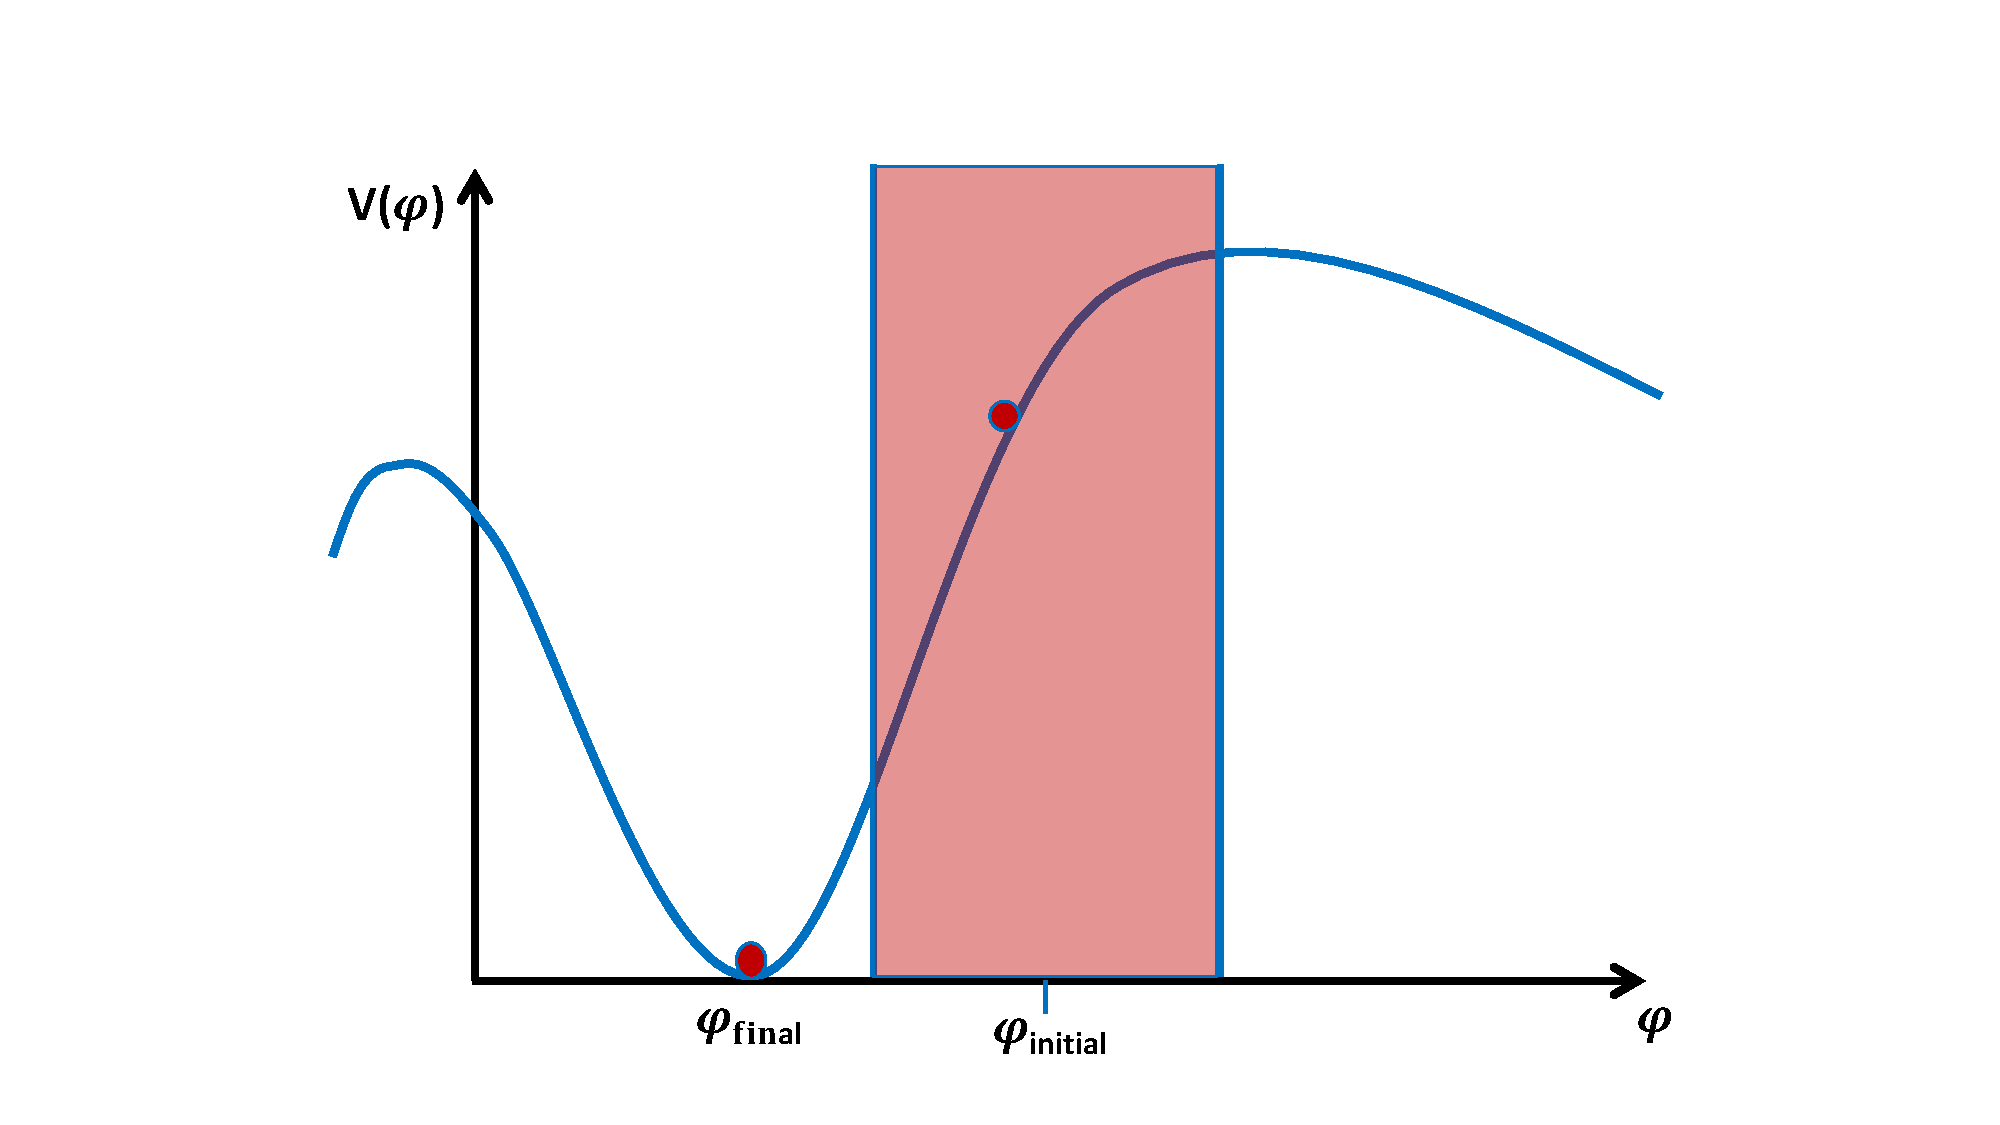
\includegraphics[width = 0.7\textwidth]{Sections/Figures/Oscillon1.pdf} 
    \caption{Non-linear effects giving rise to oscillons.}
    \label{fig:Oscillons}
\end{figure}


Neglecting gravity ($\Lambda \ll M_{\rm Pl}$) oscillons can be formed  by {\it tachyonic reheating} with tachyonic oscillations for which the homogeneous field starts oscillating in the region where $V''<0$ (since the term tachyonic) and then the modes for which $\frac{k^2}{a^2(t)}+V''(\phi(t))<0$ will grow exponentially as it can be seen from the equation for the perturbations.

A second source for exponential growth of perturbations is {\it parametric resonance} for which the perturbation frequency $\omega^2_k=k^2/a^2+V''$ varies non-adiabatically ($|\dot\omega_k/\omega_k^2|<<1 $ is violated).

It is natural to ask if the scalar potentials computed from string compactifications such as KKLT and LVS models allow for the existence of oscillons and/or oscillatons. This has been done for oscillons in \cite{Antusch:2017flz} where it was found that oscillons can be formed in KKLT scenarios, as well as for blow-up modes in the LVS scenario (see Fig.~\ref{fig:Oscillons2}). For KKLT the mechanism is parametric resonance whereas for blow-up modes the mechanism is tachyonic oscillations. Large moduli, like the volume modulus or fibre moduli do not give rise to oscillons. For KKLT and blow-up modes the spectrum for gravitational waves was computed and found to be substantially different in both cases. In principle, gravitational waves (GW) could allow us to {\it hear the shape and size of the extra dimensions} by measuring the GW spectrum. However, the frequencies obtained naturally fall in the Giga Hertz regime, far beyond the reach of Earth interferometers such as LIGO and VIRGO and any future experiments which probe frequencies below the kilo Hertz (and also outside the range of LISA \cite{amaroseoane2017laser} or future space interferometers which will probe even smaller frequencies). 
\begin{figure}[ht]
    \centering
    \includegraphics[width = 0.7\textwidth]{Sections/Figures/Oscillons3D.pdf} 
    \caption{3D modelling of oscillons for KKLT and blow-up in LVS.}
    \label{fig:Oscillons2}
\end{figure}

Such stringy oscillons are one of a large number of potential sources of gravitational waves of ultra high frequencies (UHF-GWs) at MHz range and above (see Fig.~\ref{fig:Oscillons3} for an example in KKLT and LVS models). Other sources are cosmic strings, phase transitions, preheating, boson stars, etc. Essentially, every model beyond the Standard Model may predict sources of GWs at high frequencies, with higher-energy processes giving higher frequencies (a rough rule of thumb is that GUT scale energies $10^{17}$ GeV correspond to GHz frequencies). Furthermore, usually the higher the frequency the smaller the potential experiment to detect them. However, the required sensibility (measured by the strain of the spectrum) increases with energies and therefore it is more challenging to detect them.  On the other hand, contrary to lower frequencies, there are no standard astrophysical sources at such frequencies and 
therefore any observation would imply either exotic astrophysics or a stochastic background of GWs with cosmological origin, hinting at physics beyond the Standard Model and early universe cosmology \cite{Ringwald:2020ist,Muia:2023wru}. This opens-up an interesting new challenge towards devising ways to search for UHF-GWs  (for a general discussion see \cite{Aggarwal:2020olq}; it is worth noticing that, even though there are many sources of UHF-GWs, see Fig.~\ref{fig:UHFGW},  it was the study of string cosmology that gave rise to this initiative).
\begin{figure}[ht]
    \centering
    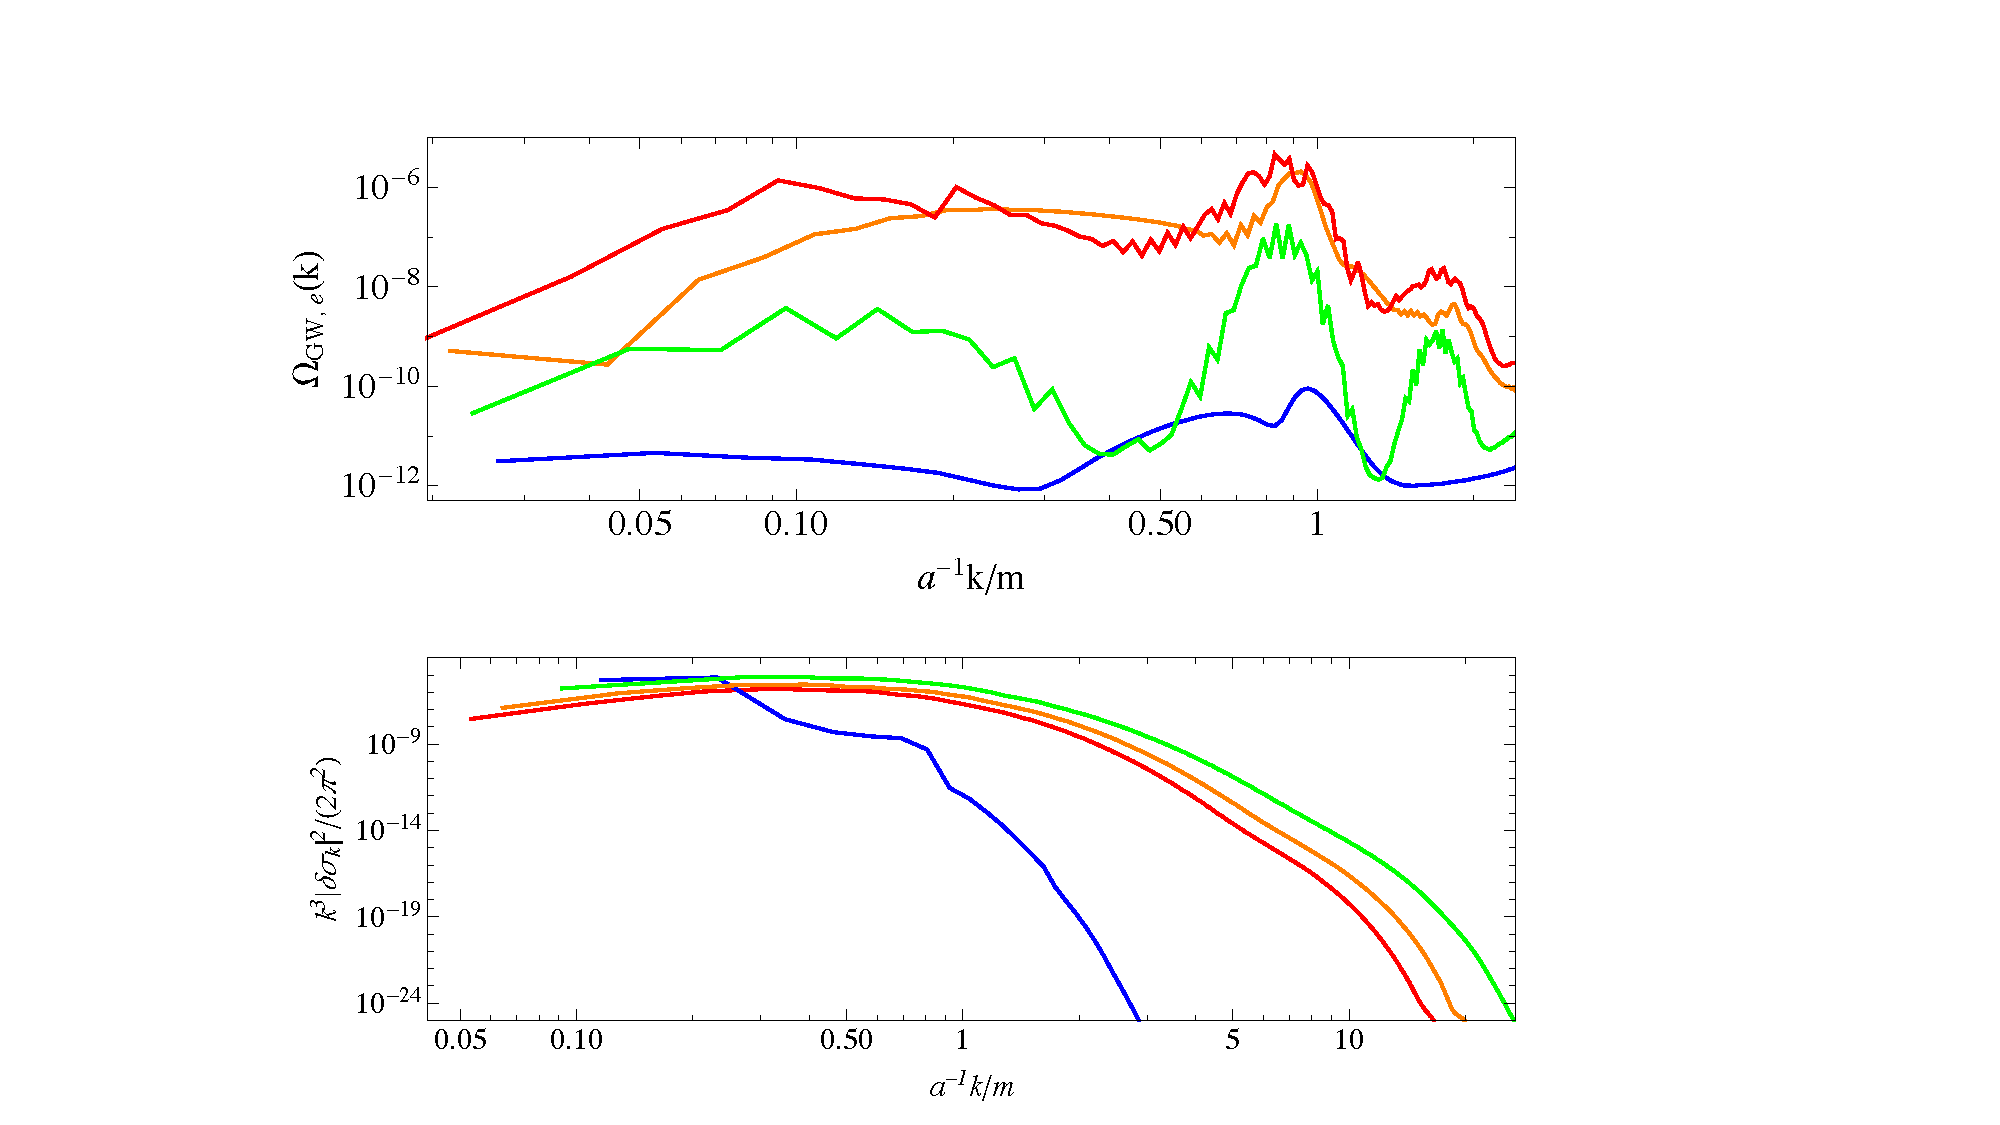
\includegraphics[width = 0.8\textwidth]{Sections/Figures/OscillonsSpectrum.pdf} 
    \caption{Spectrum of GWs for KKLT and blow-up modes in  LVS at different moments in time \cite{Antusch:2017flz}. Even though  in both cases the gravitational waves are in the Giga Hertz range, the spectrum is different for different fields and scenarios. In principle potential observation of high frequency gravitational waves can differentiate among different scenarios.  }
    \label{fig:Oscillons3}
\end{figure}

For boson stars/oscillatons there is also the possibility that the inhomogeneities collapse to black holes. A full study of the Einstein-Klein-Gordon equations needs to be studied and recently developed codes for numerical relativity, such as GRChombo \cite{Andrade:2021rbd}, have been used to explore potentials like KKLT and LVS but also potentials appearing in axion monodromy. The growth in the energy density may lead in some cases to gravitational collapse and the production of primordial black holes. This is an interesting avenue of string cosmology that is only starting to be developed \cite{Krippendorf:2018tei, Muia:2019coe, Nazari:2020fmk}.

\begin{figure}[H]
    \centering
    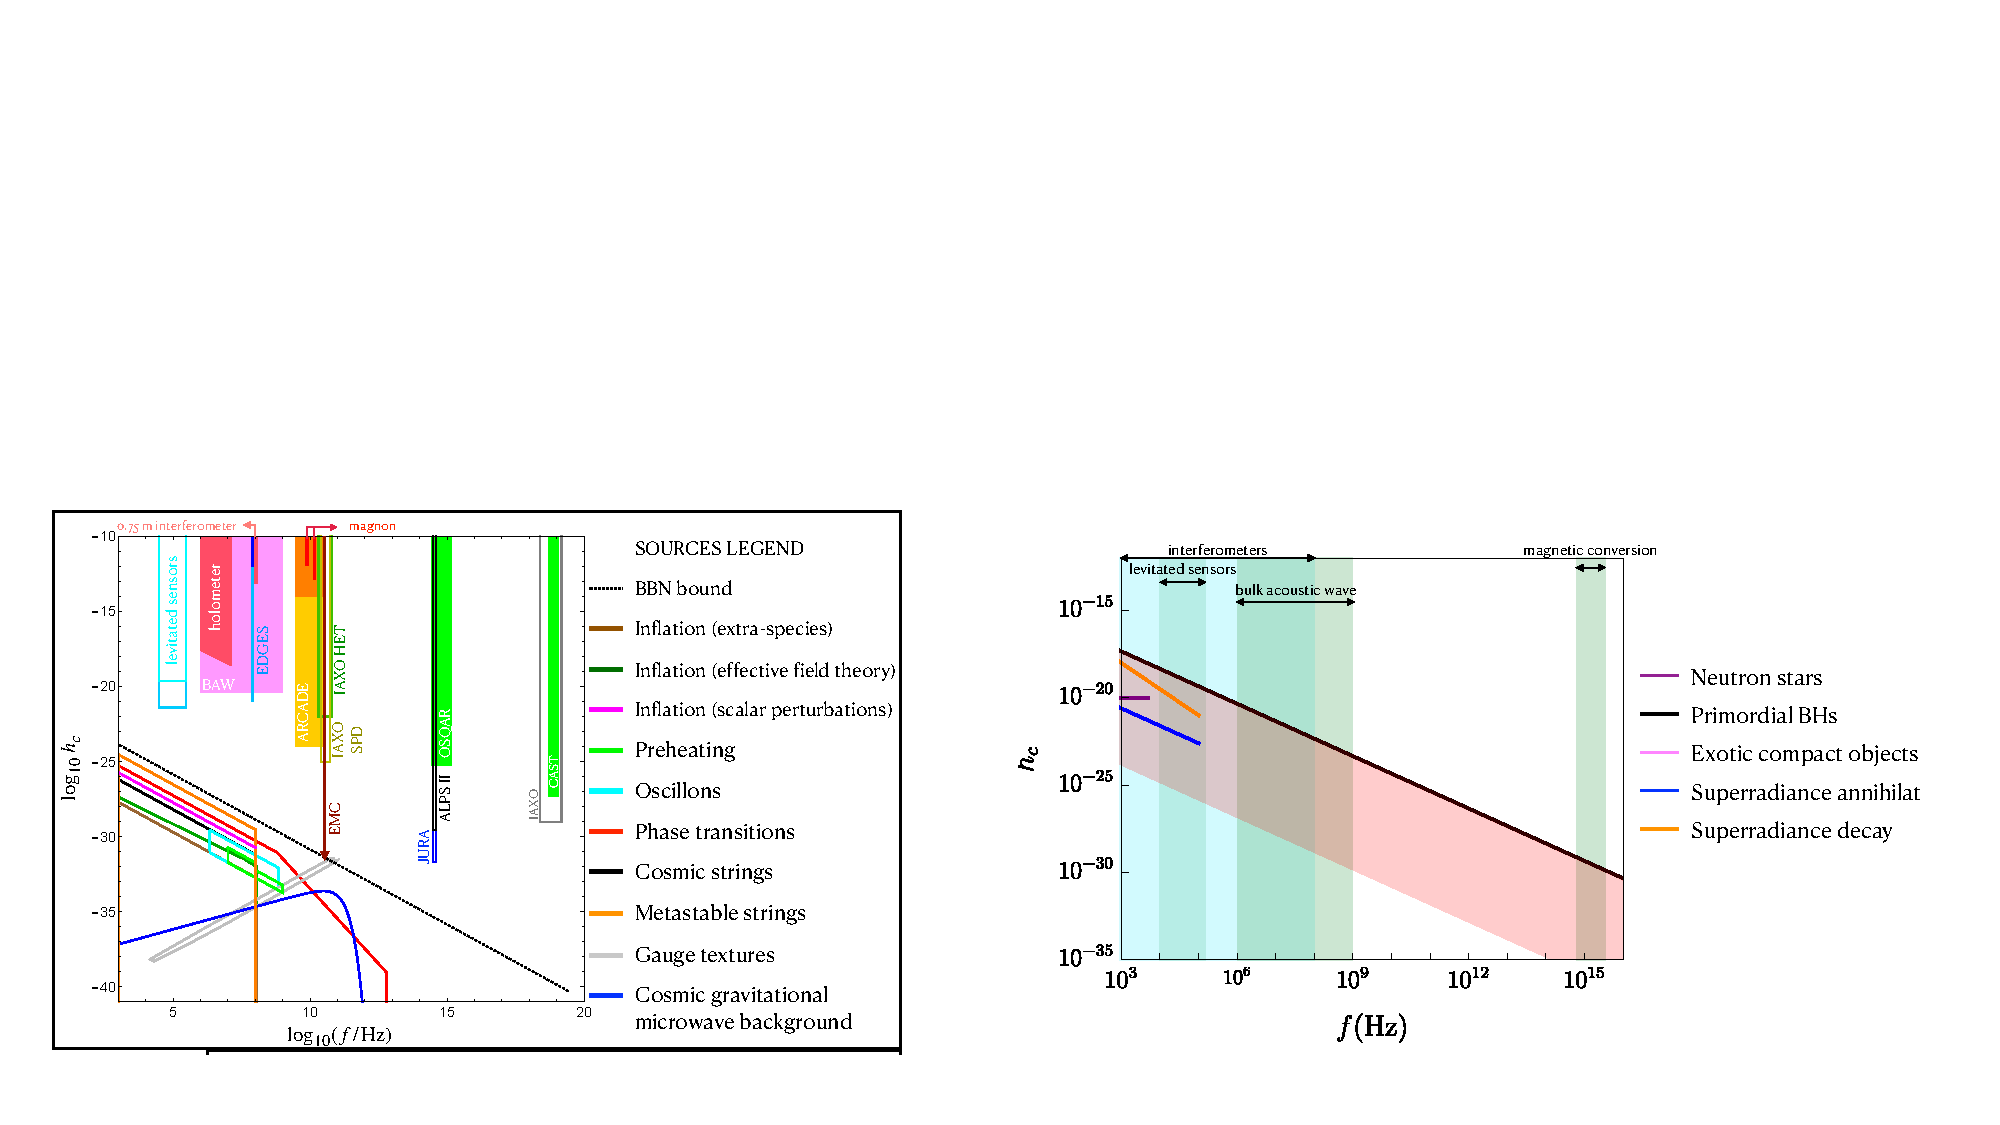
\includegraphics[width = 1.1\textwidth]{Sections/Figures/UHF-GW.pdf} 
    \caption{Different sources of high frequency gravitational waves and the experimental constraints. Taken from \cite{Aggarwal:2020olq}.}
    \label{fig:UHFGW}
\end{figure}

\subsection{Cosmic Strings and Superstrings}
% 

String theory is normally regarded as a theory of small scales and early times. However, there is one potential enormous exception to this: the possibility of a network of fundamental cosmic superstrings (or D1-strings) that stretch across the sky. For a long time, cosmic strings were regarded alongside inflation as one of the leading candidates to explain the origin of structure; in a field theory they have a natural origin as topological defects formed during processes of symmetry breaking in the early universe (as first described by Kibble in the 1970's \cite{Kibble:1976sj}).\footnote{One of the authors (JC) would like to note here that the town he lives in, Didcot, has streets named after Dirac, Higgs and Kibble.} Cosmic string were also appealing as a possible source of structure in the universe \cite{Zeldovich:1980gh, Vilenkin:1981iu}. Although observations of acoustic peaks in the CMB subsequently disfavoured cosmic strings as the primary source of structure in the universe, cosmic string networks could still exist at a subdominant level (CMB bounds on cosmic strings are described in \cite{Planck:2013mgr}).

Cosmic strings are, by convention, parametrised by a tension $G \mu$ (with $c=1$ and $G$ Newton's constant; although we normally use $\Mp$ in this review, here we conform to the standard convention for cosmic strings). 
Cosmic strings lose energy through radiation of gravitational waves and other light particles, forming a cosmic string network characterised by a scaling solution. These scaling solutions maintain a constant fraction of energy density in string relative to the overall universe during both matter and radiation epochs, with
\begin{equation}
\setlength\fboxsep{0.25cm}
\setlength\fboxrule{0.4pt}
\boxed{
\rho_{string} = \lambda \, G \mu \, \rho_{total},
}
\end{equation}
where $\lambda$ is an $\mathcal{O}(1 - 10)$ constant whose precise values depends on 
the detailed description of the network, and the possible energy loss channels. This is a complicated numerical problem (e.g. see \cite{Hindmarsh:1994re} for an older review and \cite{Gorghetto:2018myk} for more recent work). Observational bounds from potential modifications of the CMB power spectrum constrain
\begin{equation}
\setlength\fboxsep{0.25cm}
\setlength\fboxrule{0.4pt}
\boxed{
G \mu \lesssim 10^{-7}.
}
\end{equation}
The possibility of a cosmic string network consisting of fundamental strings was first considered in \cite{Witten:1984eb} with a negative conclusion: observational bounds on the tension of cosmic strings are incompatible with $ m_s \sim \Mp$ (and hence $\mu \sim G^{-1}$), and in the heterotic models then in vogue it is not possible to decouple the string and the Planck scales.

This conclusion has had to be revisited with the development of scenarios in which the fundamental string scale can be much less than the 4-dimensional Planck scale (such as in warped compactifications or in large volume compactifications such as LVS). For such models, there is no kinematic difficulty with the constraint $G \mu \lesssim 10^{-7}$: this bound is automatically satisfied in phenomenologically appealing versions of these scenarios.

Although this greatly ameliorates the kinematic constraints on the existence of networks of fundamental cosmic superstrings, one still needs a dynamical production mechanism. 
%
The most appealing such mechanism is brane-antibrane annihilation at the end of a period of brane inflation, which can lead to the formation of both D1-branes (i.e. D-strings) and fundamental strings, with $G\mu$ in the interesting range 
\be
10^{-12}\lesssim G\mu \lesssim 10^{-6}\,,
\ee
as discussed in \cite{Sarangi:2002yt, Jones:2003da}.
Cosmic string networks can only survive if the strings are themselves stable and do not immediately fragment or decay; a detailed analysis of such stability questions for cosmic superstrings is \cite{Copeland:2003bj}.
%
Cosmic strings are appealing both as a possible subdominant contribution to the energy density of the universe and 
possibly as  the sole available opportunity for the direct discovery of  macroscopic fundamental strings. 
One of the most promising routes by which cosmic (super)strings may be discovered is via gravitational radiation emitted from cusps, kinks or junctions, which may be detectable by future experiments, such as LISA \cite{amaroseoane2017laser}, and may be able to  detect loops with tensions as low as $G\mu \gtrsim 10^{-13}$ \cite{Damour:2000wa,Damour:2001bk,Damour:2004kw,Siemens:2006vk,Polchinski:2007qc}.  
Cosmic strings from a fundamental origin on the other hand, may be distinguishable from gauge theory cosmic strings by their network properties. 
For example, the reconnection probability $p$ of intersecting F- or D-strings might be much smaller than one, in contrast with ordinary strings, which have $p=1$ \cite{Jackson:2004zg}. Other effects due to (warped) extra dimensions on string evolution can help distinguish between standard and fundamental strings (see e.g.~\cite{Avgoustidis:2004zt,Blanco-Pillado:2005uwc,Avgoustidis:2007ju,OCallaghan:2010mtk,OCallaghan:2010jrm,Avgoustidis:2012vc}).
%
%%%
For further details, we refer the reader to the excellent dedicated reviews of cosmic strings and their properties \cite{Hindmarsh:1994re, Polchinski:2004ia, Copeland:2009ga}.

\newpage


